\documentclass[a4paper]{book}
\usepackage{a4wide}
\usepackage{makeidx}
\usepackage{graphicx}
\usepackage{multicol}
\usepackage{float}
\usepackage{listings}
\usepackage{color}
\usepackage{textcomp}
\usepackage{alltt}
\usepackage{times}
\usepackage{ifpdf}
\ifpdf
\usepackage[pdftex,
            pagebackref=true,
            colorlinks=true,
            linkcolor=blue,
            unicode
           ]{hyperref}
\else
\usepackage[ps2pdf,
            pagebackref=true,
            colorlinks=true,
            linkcolor=blue,
            unicode
           ]{hyperref}
\usepackage{pspicture}
\fi
\usepackage[utf8]{inputenc}
\usepackage{doxygen}
\lstset{language=C++,inputencoding=utf8,basicstyle=\footnotesize,breaklines=true,breakatwhitespace=true,tabsize=8,numbers=left }
\makeindex
\setcounter{tocdepth}{3}
\renewcommand{\footrulewidth}{0.4pt}
\begin{document}
\hypersetup{pageanchor=false}
\begin{titlepage}
\vspace*{7cm}
\begin{center}
{\Large APP\_\-TEMPLATE \\[1ex]\large 0.1 }\\
\vspace*{1cm}
{\large Generated by Doxygen 1.6.1}\\
\vspace*{0.5cm}
{\small Sat Apr 1 01:57:46 2017}\\
\end{center}
\end{titlepage}
\clearemptydoublepage
\pagenumbering{roman}
\tableofcontents
\clearemptydoublepage
\pagenumbering{arabic}
\hypersetup{pageanchor=true}
\chapter{Class Index}
\section{Class Hierarchy}
This inheritance list is sorted roughly, but not completely, alphabetically:\begin{DoxyCompactList}
\item \contentsline{section}{CL\_\-Cuda::BAR1\_\-BUF}{\pageref{structCL__Cuda_1_1BAR1__BUF}}{}
\item \contentsline{section}{CL\_\-Cuda}{\pageref{classCL__Cuda}}{}
\item \contentsline{section}{CL\_\-Cuda\_\-private}{\pageref{classCL__Cuda__private}}{}
\item \contentsline{section}{gpudma\_\-lock\_\-t}{\pageref{structgpudma__lock__t}}{}
\item \contentsline{section}{gpudma\_\-state\_\-t}{\pageref{structgpudma__state__t}}{}
\item \contentsline{section}{gpudma\_\-unlock\_\-t}{\pageref{structgpudma__unlock__t}}{}
\item \contentsline{section}{TaskBufferStatus}{\pageref{structTaskBufferStatus}}{}
\item \contentsline{section}{TaskCheckData}{\pageref{structTaskCheckData}}{}
\item \contentsline{section}{TaskData}{\pageref{structTaskData}}{}
\item \contentsline{section}{TaskMonitor}{\pageref{structTaskMonitor}}{}
\item \contentsline{section}{TF\_\-Test}{\pageref{classTF__Test}}{}
\begin{DoxyCompactList}
\item \contentsline{section}{TF\_\-TestThread}{\pageref{classTF__TestThread}}{}
\begin{DoxyCompactList}
\item \contentsline{section}{TF\_\-TestCnt}{\pageref{classTF__TestCnt}}{}
\end{DoxyCompactList}
\end{DoxyCompactList}
\end{DoxyCompactList}

\chapter{Class Index}
\section{Class List}
Here are the classes, structs, unions and interfaces with brief descriptions:\begin{DoxyCompactList}
\item\contentsline{section}{\hyperlink{structCL__Cuda_1_1BAR1__BUF}{CL\_\-Cuda::BAR1\_\-BUF} (Description buffer in BAR1 space )}{\pageref{structCL__Cuda_1_1BAR1__BUF}}{}
\item\contentsline{section}{\hyperlink{classCL__Cuda}{CL\_\-Cuda} (Common actions for CUDA device )}{\pageref{classCL__Cuda}}{}
\item\contentsline{section}{\hyperlink{classCL__Cuda__private}{CL\_\-Cuda\_\-private} (Private data for \hyperlink{classCL__Cuda}{CL\_\-Cuda} class )}{\pageref{classCL__Cuda__private}}{}
\item\contentsline{section}{\hyperlink{structgpudma__lock__t}{gpudma\_\-lock\_\-t} }{\pageref{structgpudma__lock__t}}{}
\item\contentsline{section}{\hyperlink{structgpudma__state__t}{gpudma\_\-state\_\-t} }{\pageref{structgpudma__state__t}}{}
\item\contentsline{section}{\hyperlink{structgpudma__unlock__t}{gpudma\_\-unlock\_\-t} }{\pageref{structgpudma__unlock__t}}{}
\item\contentsline{section}{\hyperlink{structTaskBufferStatus}{TaskBufferStatus} (Struct for status calculate )}{\pageref{structTaskBufferStatus}}{}
\item\contentsline{section}{\hyperlink{structTaskCheckData}{TaskCheckData} (Struct for check data in one task for one buffer )}{\pageref{structTaskCheckData}}{}
\item\contentsline{section}{\hyperlink{structTaskData}{TaskData} (Collection data for \hyperlink{classTF__TestCnt}{TF\_\-TestCnt} )}{\pageref{structTaskData}}{}
\item\contentsline{section}{\hyperlink{structTaskMonitor}{TaskMonitor} (Struct of data in monitor area in BAR1 )}{\pageref{structTaskMonitor}}{}
\item\contentsline{section}{\hyperlink{classTF__Test}{TF\_\-Test} (Base class for testing device )}{\pageref{classTF__Test}}{}
\item\contentsline{section}{\hyperlink{classTF__TestCnt}{TF\_\-TestCnt} (Checking the transmission counter at CUDA device )}{\pageref{classTF__TestCnt}}{}
\item\contentsline{section}{\hyperlink{classTF__TestThread}{TF\_\-TestThread} (Base class for application with thread )}{\pageref{classTF__TestThread}}{}
\end{DoxyCompactList}

\chapter{File Index}
\section{File List}
Here is a list of all files with brief descriptions:\begin{DoxyCompactList}
\item\contentsline{section}{common/\hyperlink{gpumemioctl_8h}{gpumemioctl.h} }{\pageref{gpumemioctl_8h}}{}
\item\contentsline{section}{common/\hyperlink{utypes_8h}{utypes.h} }{\pageref{utypes_8h}}{}
\item\contentsline{section}{common/\hyperlink{utypes__linux_8h}{utypes\_\-linux.h} }{\pageref{utypes__linux_8h}}{}
\item\contentsline{section}{cuda/\hyperlink{check__counter_8cu}{check\_\-counter.cu} }{\pageref{check__counter_8cu}}{}
\item\contentsline{section}{cuda/\hyperlink{simplePrintf_8cu}{simplePrintf.cu} }{\pageref{simplePrintf_8cu}}{}
\item\contentsline{section}{host/\hyperlink{cl__cuda_8cu}{cl\_\-cuda.cu} }{\pageref{cl__cuda_8cu}}{}
\item\contentsline{section}{host/\hyperlink{cl__cuda_8h}{cl\_\-cuda.h} }{\pageref{cl__cuda_8h}}{}
\item\contentsline{section}{host/\hyperlink{cl__cuda__test_8cpp}{cl\_\-cuda\_\-test.cpp} }{\pageref{cl__cuda__test_8cpp}}{}
\item\contentsline{section}{host/\hyperlink{main_8cpp}{main.cpp} }{\pageref{main_8cpp}}{}
\item\contentsline{section}{host/\hyperlink{run__cuda_8cu}{run\_\-cuda.cu} }{\pageref{run__cuda_8cu}}{}
\item\contentsline{section}{host/\hyperlink{task__data_8h}{task\_\-data.h} }{\pageref{task__data_8h}}{}
\item\contentsline{section}{host/\hyperlink{tf__test_8h}{tf\_\-test.h} }{\pageref{tf__test_8h}}{}
\item\contentsline{section}{host/\hyperlink{tf__testcnt_8cpp}{tf\_\-testcnt.cpp} }{\pageref{tf__testcnt_8cpp}}{}
\item\contentsline{section}{host/\hyperlink{tf__testcnt_8h}{tf\_\-testcnt.h} }{\pageref{tf__testcnt_8h}}{}
\item\contentsline{section}{host/\hyperlink{tf__testthread_8cpp}{tf\_\-testthread.cpp} }{\pageref{tf__testthread_8cpp}}{}
\item\contentsline{section}{host/\hyperlink{tf__testthread_8h}{tf\_\-testthread.h} }{\pageref{tf__testthread_8h}}{}
\end{DoxyCompactList}

\chapter{Class Documentation}
\hypertarget{structCL__Cuda_1_1BAR1__BUF}{
\section{CL\_\-Cuda::BAR1\_\-BUF Struct Reference}
\label{structCL__Cuda_1_1BAR1__BUF}\index{CL\_\-Cuda::BAR1\_\-BUF@{CL\_\-Cuda::BAR1\_\-BUF}}
}


Description buffer in BAR1 space.  


{\ttfamily \#include $<$cl\_\-cuda.h$>$}\subsection*{Public Member Functions}
\begin{DoxyCompactItemize}
\item 
\hyperlink{structCL__Cuda_1_1BAR1__BUF_ace364e1455d4dfcd2e45ab70e310ed6a}{BAR1\_\-BUF} ()
\end{DoxyCompactItemize}
\subsection*{Public Attributes}
\begin{DoxyCompactItemize}
\item 
int \hyperlink{structCL__Cuda_1_1BAR1__BUF_a8af9f6eea7e56fddd4b787779e874adb}{id}
\begin{DoxyCompactList}\small\item\em User id for buffer. \item\end{DoxyCompactList}\item 
int \hyperlink{structCL__Cuda_1_1BAR1__BUF_a3290eaf7a39a6f8ed79829ec1b62801a}{state}
\begin{DoxyCompactList}\small\item\em Status of buffer. \item\end{DoxyCompactList}\item 
size\_\-t \hyperlink{structCL__Cuda_1_1BAR1__BUF_a9919f6ce31f58f31e93552171e1de5ea}{sizeOfBytes}
\begin{DoxyCompactList}\small\item\em Size buffer of bytes. \item\end{DoxyCompactList}\item 
int \hyperlink{structCL__Cuda_1_1BAR1__BUF_a6ea1b2d3c511faee8ddb0185b005b177}{page\_\-count}
\begin{DoxyCompactList}\small\item\em Count of pages. \item\end{DoxyCompactList}\item 
int \hyperlink{structCL__Cuda_1_1BAR1__BUF_a3199bd167acc38097fbdbe0fef227b1a}{page\_\-size}
\begin{DoxyCompactList}\small\item\em Size of page. \item\end{DoxyCompactList}\item 
void $\ast$ \hyperlink{structCL__Cuda_1_1BAR1__BUF_abf1412171544f2f49dc08f7a9075b1bf}{cuda\_\-addr}
\begin{DoxyCompactList}\small\item\em address in CUDA memory \item\end{DoxyCompactList}\item 
uint64\_\-t $\ast$ \hyperlink{structCL__Cuda_1_1BAR1__BUF_a0f74a0b65b2f431fa03a573002ca0d2f}{phy\_\-addr}
\begin{DoxyCompactList}\small\item\em Array of physical addresses of pages. \item\end{DoxyCompactList}\item 
void $\ast$$\ast$ \hyperlink{structCL__Cuda_1_1BAR1__BUF_ad9ef1f7268bdba4d4727130e2d01627e}{app\_\-addr}
\begin{DoxyCompactList}\small\item\em Array of virtual addresses of pages in the application address space. \item\end{DoxyCompactList}\end{DoxyCompactItemize}


\subsection{Detailed Description}
Description buffer in BAR1 space. 

Definition at line 30 of file cl\_\-cuda.h.

\subsection{Constructor \& Destructor Documentation}
\hypertarget{structCL__Cuda_1_1BAR1__BUF_ace364e1455d4dfcd2e45ab70e310ed6a}{
\index{CL\_\-Cuda::BAR1\_\-BUF@{CL\_\-Cuda::BAR1\_\-BUF}!BAR1\_\-BUF@{BAR1\_\-BUF}}
\index{BAR1\_\-BUF@{BAR1\_\-BUF}!CL_Cuda::BAR1_BUF@{CL\_\-Cuda::BAR1\_\-BUF}}
\subsubsection[{BAR1\_\-BUF}]{\setlength{\rightskip}{0pt plus 5cm}CL\_\-Cuda::BAR1\_\-BUF::BAR1\_\-BUF ()\hspace{0.3cm}{\ttfamily  \mbox{[}inline\mbox{]}}}}
\label{structCL__Cuda_1_1BAR1__BUF_ace364e1455d4dfcd2e45ab70e310ed6a}


Definition at line 41 of file cl\_\-cuda.h.

\subsection{Member Data Documentation}
\hypertarget{structCL__Cuda_1_1BAR1__BUF_ad9ef1f7268bdba4d4727130e2d01627e}{
\index{CL\_\-Cuda::BAR1\_\-BUF@{CL\_\-Cuda::BAR1\_\-BUF}!app\_\-addr@{app\_\-addr}}
\index{app\_\-addr@{app\_\-addr}!CL_Cuda::BAR1_BUF@{CL\_\-Cuda::BAR1\_\-BUF}}
\subsubsection[{app\_\-addr}]{\setlength{\rightskip}{0pt plus 5cm}void$\ast$$\ast$ {\bf CL\_\-Cuda::BAR1\_\-BUF::app\_\-addr}}}
\label{structCL__Cuda_1_1BAR1__BUF_ad9ef1f7268bdba4d4727130e2d01627e}


Array of virtual addresses of pages in the application address space. 

Definition at line 39 of file cl\_\-cuda.h.\hypertarget{structCL__Cuda_1_1BAR1__BUF_abf1412171544f2f49dc08f7a9075b1bf}{
\index{CL\_\-Cuda::BAR1\_\-BUF@{CL\_\-Cuda::BAR1\_\-BUF}!cuda\_\-addr@{cuda\_\-addr}}
\index{cuda\_\-addr@{cuda\_\-addr}!CL_Cuda::BAR1_BUF@{CL\_\-Cuda::BAR1\_\-BUF}}
\subsubsection[{cuda\_\-addr}]{\setlength{\rightskip}{0pt plus 5cm}void$\ast$ {\bf CL\_\-Cuda::BAR1\_\-BUF::cuda\_\-addr}}}
\label{structCL__Cuda_1_1BAR1__BUF_abf1412171544f2f49dc08f7a9075b1bf}


address in CUDA memory 

Definition at line 37 of file cl\_\-cuda.h.\hypertarget{structCL__Cuda_1_1BAR1__BUF_a8af9f6eea7e56fddd4b787779e874adb}{
\index{CL\_\-Cuda::BAR1\_\-BUF@{CL\_\-Cuda::BAR1\_\-BUF}!id@{id}}
\index{id@{id}!CL_Cuda::BAR1_BUF@{CL\_\-Cuda::BAR1\_\-BUF}}
\subsubsection[{id}]{\setlength{\rightskip}{0pt plus 5cm}int {\bf CL\_\-Cuda::BAR1\_\-BUF::id}}}
\label{structCL__Cuda_1_1BAR1__BUF_a8af9f6eea7e56fddd4b787779e874adb}


User id for buffer. 

Definition at line 32 of file cl\_\-cuda.h.\hypertarget{structCL__Cuda_1_1BAR1__BUF_a6ea1b2d3c511faee8ddb0185b005b177}{
\index{CL\_\-Cuda::BAR1\_\-BUF@{CL\_\-Cuda::BAR1\_\-BUF}!page\_\-count@{page\_\-count}}
\index{page\_\-count@{page\_\-count}!CL_Cuda::BAR1_BUF@{CL\_\-Cuda::BAR1\_\-BUF}}
\subsubsection[{page\_\-count}]{\setlength{\rightskip}{0pt plus 5cm}int {\bf CL\_\-Cuda::BAR1\_\-BUF::page\_\-count}}}
\label{structCL__Cuda_1_1BAR1__BUF_a6ea1b2d3c511faee8ddb0185b005b177}


Count of pages. 

Definition at line 35 of file cl\_\-cuda.h.\hypertarget{structCL__Cuda_1_1BAR1__BUF_a3199bd167acc38097fbdbe0fef227b1a}{
\index{CL\_\-Cuda::BAR1\_\-BUF@{CL\_\-Cuda::BAR1\_\-BUF}!page\_\-size@{page\_\-size}}
\index{page\_\-size@{page\_\-size}!CL_Cuda::BAR1_BUF@{CL\_\-Cuda::BAR1\_\-BUF}}
\subsubsection[{page\_\-size}]{\setlength{\rightskip}{0pt plus 5cm}int {\bf CL\_\-Cuda::BAR1\_\-BUF::page\_\-size}}}
\label{structCL__Cuda_1_1BAR1__BUF_a3199bd167acc38097fbdbe0fef227b1a}


Size of page. 

Definition at line 36 of file cl\_\-cuda.h.\hypertarget{structCL__Cuda_1_1BAR1__BUF_a0f74a0b65b2f431fa03a573002ca0d2f}{
\index{CL\_\-Cuda::BAR1\_\-BUF@{CL\_\-Cuda::BAR1\_\-BUF}!phy\_\-addr@{phy\_\-addr}}
\index{phy\_\-addr@{phy\_\-addr}!CL_Cuda::BAR1_BUF@{CL\_\-Cuda::BAR1\_\-BUF}}
\subsubsection[{phy\_\-addr}]{\setlength{\rightskip}{0pt plus 5cm}uint64\_\-t$\ast$ {\bf CL\_\-Cuda::BAR1\_\-BUF::phy\_\-addr}}}
\label{structCL__Cuda_1_1BAR1__BUF_a0f74a0b65b2f431fa03a573002ca0d2f}


Array of physical addresses of pages. 

Definition at line 38 of file cl\_\-cuda.h.\hypertarget{structCL__Cuda_1_1BAR1__BUF_a9919f6ce31f58f31e93552171e1de5ea}{
\index{CL\_\-Cuda::BAR1\_\-BUF@{CL\_\-Cuda::BAR1\_\-BUF}!sizeOfBytes@{sizeOfBytes}}
\index{sizeOfBytes@{sizeOfBytes}!CL_Cuda::BAR1_BUF@{CL\_\-Cuda::BAR1\_\-BUF}}
\subsubsection[{sizeOfBytes}]{\setlength{\rightskip}{0pt plus 5cm}size\_\-t {\bf CL\_\-Cuda::BAR1\_\-BUF::sizeOfBytes}}}
\label{structCL__Cuda_1_1BAR1__BUF_a9919f6ce31f58f31e93552171e1de5ea}


Size buffer of bytes. 

Definition at line 34 of file cl\_\-cuda.h.\hypertarget{structCL__Cuda_1_1BAR1__BUF_a3290eaf7a39a6f8ed79829ec1b62801a}{
\index{CL\_\-Cuda::BAR1\_\-BUF@{CL\_\-Cuda::BAR1\_\-BUF}!state@{state}}
\index{state@{state}!CL_Cuda::BAR1_BUF@{CL\_\-Cuda::BAR1\_\-BUF}}
\subsubsection[{state}]{\setlength{\rightskip}{0pt plus 5cm}int {\bf CL\_\-Cuda::BAR1\_\-BUF::state}}}
\label{structCL__Cuda_1_1BAR1__BUF_a3290eaf7a39a6f8ed79829ec1b62801a}


Status of buffer. 

Definition at line 33 of file cl\_\-cuda.h.

The documentation for this struct was generated from the following file:\begin{DoxyCompactItemize}
\item 
host/\hyperlink{cl__cuda_8h}{cl\_\-cuda.h}\end{DoxyCompactItemize}

\hypertarget{classCL__Cuda}{
\section{CL\_\-Cuda Class Reference}
\label{classCL__Cuda}\index{CL\_\-Cuda@{CL\_\-Cuda}}
}


Common actions for CUDA device.  


{\ttfamily \#include $<$cl\_\-cuda.h$>$}\subsection*{Classes}
\begin{DoxyCompactItemize}
\item 
struct \hyperlink{structCL__Cuda_1_1BAR1__BUF}{BAR1\_\-BUF}
\begin{DoxyCompactList}\small\item\em Description buffer in BAR1 space. \item\end{DoxyCompactList}\end{DoxyCompactItemize}
\subsection*{Public Member Functions}
\begin{DoxyCompactItemize}
\item 
\hyperlink{classCL__Cuda_a430d5739977a8d1dcce312be2b1badae}{CL\_\-Cuda} (int argc, char $\ast$$\ast$argv)
\begin{DoxyCompactList}\small\item\em Constructor. \item\end{DoxyCompactList}\item 
virtual \hyperlink{classCL__Cuda_a3dd61a25d699f50fbe4b1891537d73e1}{$\sim$CL\_\-Cuda} ()
\item 
void \hyperlink{classCL__Cuda_a2c2b6f65ee2226a8a11052a84fcebf83}{AllocateBar1Buffer} (int sizeOfKb, \hyperlink{structCL__Cuda_1_1BAR1__BUF}{BAR1\_\-BUF} $\ast$pAdr)
\begin{DoxyCompactList}\small\item\em Allocate buffer in CUDA memory and map it in BAR1 space. \item\end{DoxyCompactList}\item 
void \hyperlink{classCL__Cuda_a2a9874acb9297efde377249468efa043}{FreeBar1Buffer} (\hyperlink{structCL__Cuda_1_1BAR1__BUF}{BAR1\_\-BUF} $\ast$pAdr)
\begin{DoxyCompactList}\small\item\em Release buffer from BAR1 space and from CUDA memory. \item\end{DoxyCompactList}\end{DoxyCompactItemize}
\subsection*{Private Attributes}
\begin{DoxyCompactItemize}
\item 
\hyperlink{classCL__Cuda__private}{CL\_\-Cuda\_\-private} $\ast$ \hyperlink{classCL__Cuda_ac829b1e46585219ac2c30ccab6e7c9f8}{pd}
\end{DoxyCompactItemize}


\subsection{Detailed Description}
Common actions for CUDA device. 

Definition at line 19 of file cl\_\-cuda.h.

\subsection{Constructor \& Destructor Documentation}
\hypertarget{classCL__Cuda_a430d5739977a8d1dcce312be2b1badae}{
\index{CL\_\-Cuda@{CL\_\-Cuda}!CL\_\-Cuda@{CL\_\-Cuda}}
\index{CL\_\-Cuda@{CL\_\-Cuda}!CL_Cuda@{CL\_\-Cuda}}
\subsubsection[{CL\_\-Cuda}]{\setlength{\rightskip}{0pt plus 5cm}CL\_\-Cuda::CL\_\-Cuda (int {\em argc}, \/  char $\ast$$\ast$ {\em argv})}}
\label{classCL__Cuda_a430d5739977a8d1dcce312be2b1badae}


Constructor. 
\begin{DoxyParams}{Parameters}
\item[{\em argc}]argc from main function \item[{\em argv}]argv from main function \end{DoxyParams}


Definition at line 67 of file cl\_\-cuda.cu.\hypertarget{classCL__Cuda_a3dd61a25d699f50fbe4b1891537d73e1}{
\index{CL\_\-Cuda@{CL\_\-Cuda}!$\sim$CL\_\-Cuda@{$\sim$CL\_\-Cuda}}
\index{$\sim$CL\_\-Cuda@{$\sim$CL\_\-Cuda}!CL_Cuda@{CL\_\-Cuda}}
\subsubsection[{$\sim$CL\_\-Cuda}]{\setlength{\rightskip}{0pt plus 5cm}CL\_\-Cuda::$\sim$CL\_\-Cuda ()\hspace{0.3cm}{\ttfamily  \mbox{[}virtual\mbox{]}}}}
\label{classCL__Cuda_a3dd61a25d699f50fbe4b1891537d73e1}


Definition at line 125 of file cl\_\-cuda.cu.

\subsection{Member Function Documentation}
\hypertarget{classCL__Cuda_a2c2b6f65ee2226a8a11052a84fcebf83}{
\index{CL\_\-Cuda@{CL\_\-Cuda}!AllocateBar1Buffer@{AllocateBar1Buffer}}
\index{AllocateBar1Buffer@{AllocateBar1Buffer}!CL_Cuda@{CL\_\-Cuda}}
\subsubsection[{AllocateBar1Buffer}]{\setlength{\rightskip}{0pt plus 5cm}void CL\_\-Cuda::AllocateBar1Buffer (int {\em sizeOfKb}, \/  {\bf BAR1\_\-BUF} $\ast$ {\em pAdr})}}
\label{classCL__Cuda_a2c2b6f65ee2226a8a11052a84fcebf83}


Allocate buffer in CUDA memory and map it in BAR1 space. 

Definition at line 133 of file cl\_\-cuda.cu.\hypertarget{classCL__Cuda_a2a9874acb9297efde377249468efa043}{
\index{CL\_\-Cuda@{CL\_\-Cuda}!FreeBar1Buffer@{FreeBar1Buffer}}
\index{FreeBar1Buffer@{FreeBar1Buffer}!CL_Cuda@{CL\_\-Cuda}}
\subsubsection[{FreeBar1Buffer}]{\setlength{\rightskip}{0pt plus 5cm}void CL\_\-Cuda::FreeBar1Buffer ({\bf BAR1\_\-BUF} $\ast$ {\em pAdr})}}
\label{classCL__Cuda_a2a9874acb9297efde377249468efa043}


Release buffer from BAR1 space and from CUDA memory. 

Definition at line 245 of file cl\_\-cuda.cu.

\subsection{Member Data Documentation}
\hypertarget{classCL__Cuda_ac829b1e46585219ac2c30ccab6e7c9f8}{
\index{CL\_\-Cuda@{CL\_\-Cuda}!pd@{pd}}
\index{pd@{pd}!CL_Cuda@{CL\_\-Cuda}}
\subsubsection[{pd}]{\setlength{\rightskip}{0pt plus 5cm}{\bf CL\_\-Cuda\_\-private}$\ast$ {\bf CL\_\-Cuda::pd}\hspace{0.3cm}{\ttfamily  \mbox{[}private\mbox{]}}}}
\label{classCL__Cuda_ac829b1e46585219ac2c30ccab6e7c9f8}


Definition at line 23 of file cl\_\-cuda.h.

The documentation for this class was generated from the following files:\begin{DoxyCompactItemize}
\item 
host/\hyperlink{cl__cuda_8h}{cl\_\-cuda.h}\item 
host/\hyperlink{cl__cuda_8cu}{cl\_\-cuda.cu}\end{DoxyCompactItemize}

\hypertarget{classCL__Cuda__private}{
\section{CL\_\-Cuda\_\-private Class Reference}
\label{classCL__Cuda__private}\index{CL\_\-Cuda\_\-private@{CL\_\-Cuda\_\-private}}
}


Private data for \hyperlink{classCL__Cuda}{CL\_\-Cuda} class.  
\subsection*{Public Attributes}
\begin{DoxyCompactItemize}
\item 
int \hyperlink{classCL__Cuda__private_ac48da65acdaf7d7400a98a6d2f893f1e}{devID}
\begin{DoxyCompactList}\small\item\em Id for CUDA device. \item\end{DoxyCompactList}\item 
cudaDeviceProp \hyperlink{classCL__Cuda__private_ad7b57a953847c106179d0b0504111fb3}{props}
\begin{DoxyCompactList}\small\item\em attributes for CUDA device \item\end{DoxyCompactList}\item 
int \hyperlink{classCL__Cuda__private_a35f342c3bcf3de609aa03c2d1c8665a4}{fd}
\begin{DoxyCompactList}\small\item\em description of gpumem driver \item\end{DoxyCompactList}\item 
CUdevice \hyperlink{classCL__Cuda__private_a8743e6aaa2155f6695cd8165f07f8225}{device}
\begin{DoxyCompactList}\small\item\em Descriptor CUDA device. \item\end{DoxyCompactList}\item 
char \hyperlink{classCL__Cuda__private_a3f0394a7cd0f0e7542e9f33252eca8b6}{name} \mbox{[}256\mbox{]}
\begin{DoxyCompactList}\small\item\em Name of CUDA device. \item\end{DoxyCompactList}\item 
int \hyperlink{classCL__Cuda__private_a9cc50a203aee2dec568464e102f4cb54}{major}
\item 
int \hyperlink{classCL__Cuda__private_a7b640660cd0e6b853d6a1e8d57d9f9dc}{minor}
\begin{DoxyCompactList}\small\item\em Capability numbers;. \item\end{DoxyCompactList}\item 
size\_\-t \hyperlink{classCL__Cuda__private_a66237a60653b0a5c1fe4fd21bb688da2}{global\_\-mem}
\begin{DoxyCompactList}\small\item\em Size of memory on CUDA device. \item\end{DoxyCompactList}\item 
CUcontext \hyperlink{classCL__Cuda__private_a5cee71c336fd132e3030dd02045eef43}{context}
\begin{DoxyCompactList}\small\item\em Contex for all cuda functions. \item\end{DoxyCompactList}\end{DoxyCompactItemize}


\subsection{Detailed Description}
Private data for \hyperlink{classCL__Cuda}{CL\_\-Cuda} class. 

Definition at line 44 of file cl\_\-cuda.cu.

\subsection{Member Data Documentation}
\hypertarget{classCL__Cuda__private_a5cee71c336fd132e3030dd02045eef43}{
\index{CL\_\-Cuda\_\-private@{CL\_\-Cuda\_\-private}!context@{context}}
\index{context@{context}!CL_Cuda_private@{CL\_\-Cuda\_\-private}}
\subsubsection[{context}]{\setlength{\rightskip}{0pt plus 5cm}CUcontext {\bf CL\_\-Cuda\_\-private::context}}}
\label{classCL__Cuda__private_a5cee71c336fd132e3030dd02045eef43}


Contex for all cuda functions. 

Definition at line 57 of file cl\_\-cuda.cu.\hypertarget{classCL__Cuda__private_a8743e6aaa2155f6695cd8165f07f8225}{
\index{CL\_\-Cuda\_\-private@{CL\_\-Cuda\_\-private}!device@{device}}
\index{device@{device}!CL_Cuda_private@{CL\_\-Cuda\_\-private}}
\subsubsection[{device}]{\setlength{\rightskip}{0pt plus 5cm}CUdevice {\bf CL\_\-Cuda\_\-private::device}}}
\label{classCL__Cuda__private_a8743e6aaa2155f6695cd8165f07f8225}


Descriptor CUDA device. 

Definition at line 53 of file cl\_\-cuda.cu.\hypertarget{classCL__Cuda__private_ac48da65acdaf7d7400a98a6d2f893f1e}{
\index{CL\_\-Cuda\_\-private@{CL\_\-Cuda\_\-private}!devID@{devID}}
\index{devID@{devID}!CL_Cuda_private@{CL\_\-Cuda\_\-private}}
\subsubsection[{devID}]{\setlength{\rightskip}{0pt plus 5cm}int {\bf CL\_\-Cuda\_\-private::devID}}}
\label{classCL__Cuda__private_ac48da65acdaf7d7400a98a6d2f893f1e}


Id for CUDA device. 

Definition at line 48 of file cl\_\-cuda.cu.\hypertarget{classCL__Cuda__private_a35f342c3bcf3de609aa03c2d1c8665a4}{
\index{CL\_\-Cuda\_\-private@{CL\_\-Cuda\_\-private}!fd@{fd}}
\index{fd@{fd}!CL_Cuda_private@{CL\_\-Cuda\_\-private}}
\subsubsection[{fd}]{\setlength{\rightskip}{0pt plus 5cm}int {\bf CL\_\-Cuda\_\-private::fd}}}
\label{classCL__Cuda__private_a35f342c3bcf3de609aa03c2d1c8665a4}


description of gpumem driver 

Definition at line 51 of file cl\_\-cuda.cu.\hypertarget{classCL__Cuda__private_a66237a60653b0a5c1fe4fd21bb688da2}{
\index{CL\_\-Cuda\_\-private@{CL\_\-Cuda\_\-private}!global\_\-mem@{global\_\-mem}}
\index{global\_\-mem@{global\_\-mem}!CL_Cuda_private@{CL\_\-Cuda\_\-private}}
\subsubsection[{global\_\-mem}]{\setlength{\rightskip}{0pt plus 5cm}size\_\-t {\bf CL\_\-Cuda\_\-private::global\_\-mem}}}
\label{classCL__Cuda__private_a66237a60653b0a5c1fe4fd21bb688da2}


Size of memory on CUDA device. 

Definition at line 56 of file cl\_\-cuda.cu.\hypertarget{classCL__Cuda__private_a9cc50a203aee2dec568464e102f4cb54}{
\index{CL\_\-Cuda\_\-private@{CL\_\-Cuda\_\-private}!major@{major}}
\index{major@{major}!CL_Cuda_private@{CL\_\-Cuda\_\-private}}
\subsubsection[{major}]{\setlength{\rightskip}{0pt plus 5cm}int {\bf CL\_\-Cuda\_\-private::major}}}
\label{classCL__Cuda__private_a9cc50a203aee2dec568464e102f4cb54}


Definition at line 55 of file cl\_\-cuda.cu.\hypertarget{classCL__Cuda__private_a7b640660cd0e6b853d6a1e8d57d9f9dc}{
\index{CL\_\-Cuda\_\-private@{CL\_\-Cuda\_\-private}!minor@{minor}}
\index{minor@{minor}!CL_Cuda_private@{CL\_\-Cuda\_\-private}}
\subsubsection[{minor}]{\setlength{\rightskip}{0pt plus 5cm}int {\bf CL\_\-Cuda\_\-private::minor}}}
\label{classCL__Cuda__private_a7b640660cd0e6b853d6a1e8d57d9f9dc}


Capability numbers;. 

Definition at line 55 of file cl\_\-cuda.cu.\hypertarget{classCL__Cuda__private_a3f0394a7cd0f0e7542e9f33252eca8b6}{
\index{CL\_\-Cuda\_\-private@{CL\_\-Cuda\_\-private}!name@{name}}
\index{name@{name}!CL_Cuda_private@{CL\_\-Cuda\_\-private}}
\subsubsection[{name}]{\setlength{\rightskip}{0pt plus 5cm}char {\bf CL\_\-Cuda\_\-private::name}\mbox{[}256\mbox{]}}}
\label{classCL__Cuda__private_a3f0394a7cd0f0e7542e9f33252eca8b6}


Name of CUDA device. 

Definition at line 54 of file cl\_\-cuda.cu.\hypertarget{classCL__Cuda__private_ad7b57a953847c106179d0b0504111fb3}{
\index{CL\_\-Cuda\_\-private@{CL\_\-Cuda\_\-private}!props@{props}}
\index{props@{props}!CL_Cuda_private@{CL\_\-Cuda\_\-private}}
\subsubsection[{props}]{\setlength{\rightskip}{0pt plus 5cm}cudaDeviceProp {\bf CL\_\-Cuda\_\-private::props}}}
\label{classCL__Cuda__private_ad7b57a953847c106179d0b0504111fb3}


attributes for CUDA device 

Definition at line 49 of file cl\_\-cuda.cu.

The documentation for this class was generated from the following file:\begin{DoxyCompactItemize}
\item 
host/\hyperlink{cl__cuda_8cu}{cl\_\-cuda.cu}\end{DoxyCompactItemize}

\hypertarget{structgpudma__lock__t}{
\section{gpudma\_\-lock\_\-t Struct Reference}
\label{structgpudma__lock__t}\index{gpudma\_\-lock\_\-t@{gpudma\_\-lock\_\-t}}
}


{\ttfamily \#include $<$gpumemioctl.h$>$}\subsection*{Public Attributes}
\begin{DoxyCompactItemize}
\item 
void $\ast$ \hyperlink{structgpudma__lock__t_a759be71a976110412ebf1384131930ae}{handle}
\item 
uint64\_\-t \hyperlink{structgpudma__lock__t_a3bcf1355c5cf552d0eedbae3f829f83d}{addr}
\item 
uint64\_\-t \hyperlink{structgpudma__lock__t_a7c3c9d36171da51b60208422084474a7}{size}
\item 
size\_\-t \hyperlink{structgpudma__lock__t_a7a5449281d51204ac90b1b6803004784}{page\_\-count}
\end{DoxyCompactItemize}


\subsection{Detailed Description}


Definition at line 33 of file gpumemioctl.h.

\subsection{Member Data Documentation}
\hypertarget{structgpudma__lock__t_a3bcf1355c5cf552d0eedbae3f829f83d}{
\index{gpudma\_\-lock\_\-t@{gpudma\_\-lock\_\-t}!addr@{addr}}
\index{addr@{addr}!gpudma_lock_t@{gpudma\_\-lock\_\-t}}
\subsubsection[{addr}]{\setlength{\rightskip}{0pt plus 5cm}uint64\_\-t {\bf gpudma\_\-lock\_\-t::addr}}}
\label{structgpudma__lock__t_a3bcf1355c5cf552d0eedbae3f829f83d}


Definition at line 35 of file gpumemioctl.h.\hypertarget{structgpudma__lock__t_a759be71a976110412ebf1384131930ae}{
\index{gpudma\_\-lock\_\-t@{gpudma\_\-lock\_\-t}!handle@{handle}}
\index{handle@{handle}!gpudma_lock_t@{gpudma\_\-lock\_\-t}}
\subsubsection[{handle}]{\setlength{\rightskip}{0pt plus 5cm}void$\ast$ {\bf gpudma\_\-lock\_\-t::handle}}}
\label{structgpudma__lock__t_a759be71a976110412ebf1384131930ae}


Definition at line 34 of file gpumemioctl.h.\hypertarget{structgpudma__lock__t_a7a5449281d51204ac90b1b6803004784}{
\index{gpudma\_\-lock\_\-t@{gpudma\_\-lock\_\-t}!page\_\-count@{page\_\-count}}
\index{page\_\-count@{page\_\-count}!gpudma_lock_t@{gpudma\_\-lock\_\-t}}
\subsubsection[{page\_\-count}]{\setlength{\rightskip}{0pt plus 5cm}size\_\-t {\bf gpudma\_\-lock\_\-t::page\_\-count}}}
\label{structgpudma__lock__t_a7a5449281d51204ac90b1b6803004784}


Definition at line 37 of file gpumemioctl.h.\hypertarget{structgpudma__lock__t_a7c3c9d36171da51b60208422084474a7}{
\index{gpudma\_\-lock\_\-t@{gpudma\_\-lock\_\-t}!size@{size}}
\index{size@{size}!gpudma_lock_t@{gpudma\_\-lock\_\-t}}
\subsubsection[{size}]{\setlength{\rightskip}{0pt plus 5cm}uint64\_\-t {\bf gpudma\_\-lock\_\-t::size}}}
\label{structgpudma__lock__t_a7c3c9d36171da51b60208422084474a7}


Definition at line 36 of file gpumemioctl.h.

The documentation for this struct was generated from the following file:\begin{DoxyCompactItemize}
\item 
common/\hyperlink{gpumemioctl_8h}{gpumemioctl.h}\end{DoxyCompactItemize}

\hypertarget{structgpudma__state__t}{
\section{gpudma\_\-state\_\-t Struct Reference}
\label{structgpudma__state__t}\index{gpudma\_\-state\_\-t@{gpudma\_\-state\_\-t}}
}


{\ttfamily \#include $<$gpumemioctl.h$>$}\subsection*{Public Attributes}
\begin{DoxyCompactItemize}
\item 
void $\ast$ \hyperlink{structgpudma__state__t_a6a424759c2617a6e098369d99c780f08}{handle}
\item 
size\_\-t \hyperlink{structgpudma__state__t_a9c5c7a8c240e9baec5e666f8081417f2}{page\_\-count}
\item 
size\_\-t \hyperlink{structgpudma__state__t_a9c5a9f537eb39d78e3505ca858a14aaf}{page\_\-size}
\item 
uint64\_\-t \hyperlink{structgpudma__state__t_a7d45e0f5c232b286ca20c0a5f3e0d032}{pages} \mbox{[}1\mbox{]}
\end{DoxyCompactItemize}


\subsection{Detailed Description}


Definition at line 48 of file gpumemioctl.h.

\subsection{Member Data Documentation}
\hypertarget{structgpudma__state__t_a6a424759c2617a6e098369d99c780f08}{
\index{gpudma\_\-state\_\-t@{gpudma\_\-state\_\-t}!handle@{handle}}
\index{handle@{handle}!gpudma_state_t@{gpudma\_\-state\_\-t}}
\subsubsection[{handle}]{\setlength{\rightskip}{0pt plus 5cm}void$\ast$ {\bf gpudma\_\-state\_\-t::handle}}}
\label{structgpudma__state__t_a6a424759c2617a6e098369d99c780f08}


Definition at line 49 of file gpumemioctl.h.\hypertarget{structgpudma__state__t_a9c5c7a8c240e9baec5e666f8081417f2}{
\index{gpudma\_\-state\_\-t@{gpudma\_\-state\_\-t}!page\_\-count@{page\_\-count}}
\index{page\_\-count@{page\_\-count}!gpudma_state_t@{gpudma\_\-state\_\-t}}
\subsubsection[{page\_\-count}]{\setlength{\rightskip}{0pt plus 5cm}size\_\-t {\bf gpudma\_\-state\_\-t::page\_\-count}}}
\label{structgpudma__state__t_a9c5c7a8c240e9baec5e666f8081417f2}


Definition at line 50 of file gpumemioctl.h.\hypertarget{structgpudma__state__t_a9c5a9f537eb39d78e3505ca858a14aaf}{
\index{gpudma\_\-state\_\-t@{gpudma\_\-state\_\-t}!page\_\-size@{page\_\-size}}
\index{page\_\-size@{page\_\-size}!gpudma_state_t@{gpudma\_\-state\_\-t}}
\subsubsection[{page\_\-size}]{\setlength{\rightskip}{0pt plus 5cm}size\_\-t {\bf gpudma\_\-state\_\-t::page\_\-size}}}
\label{structgpudma__state__t_a9c5a9f537eb39d78e3505ca858a14aaf}


Definition at line 51 of file gpumemioctl.h.\hypertarget{structgpudma__state__t_a7d45e0f5c232b286ca20c0a5f3e0d032}{
\index{gpudma\_\-state\_\-t@{gpudma\_\-state\_\-t}!pages@{pages}}
\index{pages@{pages}!gpudma_state_t@{gpudma\_\-state\_\-t}}
\subsubsection[{pages}]{\setlength{\rightskip}{0pt plus 5cm}uint64\_\-t {\bf gpudma\_\-state\_\-t::pages}\mbox{[}1\mbox{]}}}
\label{structgpudma__state__t_a7d45e0f5c232b286ca20c0a5f3e0d032}


Definition at line 52 of file gpumemioctl.h.

The documentation for this struct was generated from the following file:\begin{DoxyCompactItemize}
\item 
common/\hyperlink{gpumemioctl_8h}{gpumemioctl.h}\end{DoxyCompactItemize}

\hypertarget{structgpudma__unlock__t}{
\section{gpudma\_\-unlock\_\-t Struct Reference}
\label{structgpudma__unlock__t}\index{gpudma\_\-unlock\_\-t@{gpudma\_\-unlock\_\-t}}
}


{\ttfamily \#include $<$gpumemioctl.h$>$}\subsection*{Public Attributes}
\begin{DoxyCompactItemize}
\item 
void $\ast$ \hyperlink{structgpudma__unlock__t_ad10027324aed6d13ed3e6c935c0f0787}{handle}
\end{DoxyCompactItemize}


\subsection{Detailed Description}


Definition at line 42 of file gpumemioctl.h.

\subsection{Member Data Documentation}
\hypertarget{structgpudma__unlock__t_ad10027324aed6d13ed3e6c935c0f0787}{
\index{gpudma\_\-unlock\_\-t@{gpudma\_\-unlock\_\-t}!handle@{handle}}
\index{handle@{handle}!gpudma_unlock_t@{gpudma\_\-unlock\_\-t}}
\subsubsection[{handle}]{\setlength{\rightskip}{0pt plus 5cm}void$\ast$ {\bf gpudma\_\-unlock\_\-t::handle}}}
\label{structgpudma__unlock__t_ad10027324aed6d13ed3e6c935c0f0787}


Definition at line 43 of file gpumemioctl.h.

The documentation for this struct was generated from the following file:\begin{DoxyCompactItemize}
\item 
common/\hyperlink{gpumemioctl_8h}{gpumemioctl.h}\end{DoxyCompactItemize}

\hypertarget{structTaskBufferStatus}{
\section{TaskBufferStatus Struct Reference}
\label{structTaskBufferStatus}\index{TaskBufferStatus@{TaskBufferStatus}}
}


Struct for status calculate.  


{\ttfamily \#include $<$task\_\-data.h$>$}\subsection*{Public Attributes}
\begin{DoxyCompactItemize}
\item 
unsigned int \hyperlink{structTaskBufferStatus_ad2f11a4542658ad3fdec4eac2bcf8eeb}{irqFlag}
\begin{DoxyCompactList}\small\item\em 1 -\/ ready data in bar1 buffer \item\end{DoxyCompactList}\item 
unsigned int \hyperlink{structTaskBufferStatus_aac53804036a15457af35c1a4fa0595d2}{res0}
\item 
unsigned int \hyperlink{structTaskBufferStatus_a488df55e08dfb02be4d793186efef2f0}{res1}
\item 
unsigned int \hyperlink{structTaskBufferStatus_aa37878c4c19f5cfd5bbb010c3377bd94}{blockRd}
\begin{DoxyCompactList}\small\item\em count of read buffer \item\end{DoxyCompactList}\item 
unsigned int \hyperlink{structTaskBufferStatus_aabc9f698de646935e330356dab0736c9}{blockOk}
\begin{DoxyCompactList}\small\item\em count of correct buffers \item\end{DoxyCompactList}\item 
unsigned int \hyperlink{structTaskBufferStatus_a81844ea492b32a7e9d29dda117a3f935}{blockError}
\begin{DoxyCompactList}\small\item\em count of buffer with errors \item\end{DoxyCompactList}\item 
unsigned int \hyperlink{structTaskBufferStatus_ac09e520b4c35bddd83c61ab0a0d20e94}{sizeOfKBytes}
\begin{DoxyCompactList}\small\item\em size of buffers in kilobytes \item\end{DoxyCompactList}\item 
void $\ast$ \hyperlink{structTaskBufferStatus_a530d1c73d828ba73216ab03fa67be5d4}{ptrCudaIn}
\begin{DoxyCompactList}\small\item\em pointer on bar1 buffer in the Cuda memory \item\end{DoxyCompactList}\item 
void $\ast$ \hyperlink{structTaskBufferStatus_ac3996bd365a6296309bd372b227bbbdc}{ptrCudaOut}
\begin{DoxyCompactList}\small\item\em pointer on output buffer in the Cuda memory \item\end{DoxyCompactList}\item 
\hyperlink{structTaskCheckData}{TaskCheckData} \hyperlink{structTaskBufferStatus_ab95fe846215632d00858e3ed0fa4a293}{check} \mbox{[}\hyperlink{task__data_8h_a3c397e824761613a5e1d71e1b6d49b6d}{TaskCounts}\mbox{]}
\begin{DoxyCompactList}\small\item\em current results for test one buffer \item\end{DoxyCompactList}\end{DoxyCompactItemize}


\subsection{Detailed Description}
Struct for status calculate. 

Definition at line 40 of file task\_\-data.h.

\subsection{Member Data Documentation}
\hypertarget{structTaskBufferStatus_a81844ea492b32a7e9d29dda117a3f935}{
\index{TaskBufferStatus@{TaskBufferStatus}!blockError@{blockError}}
\index{blockError@{blockError}!TaskBufferStatus@{TaskBufferStatus}}
\subsubsection[{blockError}]{\setlength{\rightskip}{0pt plus 5cm}unsigned int {\bf TaskBufferStatus::blockError}}}
\label{structTaskBufferStatus_a81844ea492b32a7e9d29dda117a3f935}


count of buffer with errors 

Definition at line 47 of file task\_\-data.h.\hypertarget{structTaskBufferStatus_aabc9f698de646935e330356dab0736c9}{
\index{TaskBufferStatus@{TaskBufferStatus}!blockOk@{blockOk}}
\index{blockOk@{blockOk}!TaskBufferStatus@{TaskBufferStatus}}
\subsubsection[{blockOk}]{\setlength{\rightskip}{0pt plus 5cm}unsigned int {\bf TaskBufferStatus::blockOk}}}
\label{structTaskBufferStatus_aabc9f698de646935e330356dab0736c9}


count of correct buffers 

Definition at line 46 of file task\_\-data.h.\hypertarget{structTaskBufferStatus_aa37878c4c19f5cfd5bbb010c3377bd94}{
\index{TaskBufferStatus@{TaskBufferStatus}!blockRd@{blockRd}}
\index{blockRd@{blockRd}!TaskBufferStatus@{TaskBufferStatus}}
\subsubsection[{blockRd}]{\setlength{\rightskip}{0pt plus 5cm}unsigned int {\bf TaskBufferStatus::blockRd}}}
\label{structTaskBufferStatus_aa37878c4c19f5cfd5bbb010c3377bd94}


count of read buffer 

Definition at line 45 of file task\_\-data.h.\hypertarget{structTaskBufferStatus_ab95fe846215632d00858e3ed0fa4a293}{
\index{TaskBufferStatus@{TaskBufferStatus}!check@{check}}
\index{check@{check}!TaskBufferStatus@{TaskBufferStatus}}
\subsubsection[{check}]{\setlength{\rightskip}{0pt plus 5cm}{\bf TaskCheckData} {\bf TaskBufferStatus::check}\mbox{[}{\bf TaskCounts}\mbox{]}}}
\label{structTaskBufferStatus_ab95fe846215632d00858e3ed0fa4a293}


current results for test one buffer 

Definition at line 53 of file task\_\-data.h.\hypertarget{structTaskBufferStatus_ad2f11a4542658ad3fdec4eac2bcf8eeb}{
\index{TaskBufferStatus@{TaskBufferStatus}!irqFlag@{irqFlag}}
\index{irqFlag@{irqFlag}!TaskBufferStatus@{TaskBufferStatus}}
\subsubsection[{irqFlag}]{\setlength{\rightskip}{0pt plus 5cm}unsigned int {\bf TaskBufferStatus::irqFlag}}}
\label{structTaskBufferStatus_ad2f11a4542658ad3fdec4eac2bcf8eeb}


1 -\/ ready data in bar1 buffer 

Definition at line 42 of file task\_\-data.h.\hypertarget{structTaskBufferStatus_a530d1c73d828ba73216ab03fa67be5d4}{
\index{TaskBufferStatus@{TaskBufferStatus}!ptrCudaIn@{ptrCudaIn}}
\index{ptrCudaIn@{ptrCudaIn}!TaskBufferStatus@{TaskBufferStatus}}
\subsubsection[{ptrCudaIn}]{\setlength{\rightskip}{0pt plus 5cm}void$\ast$ {\bf TaskBufferStatus::ptrCudaIn}}}
\label{structTaskBufferStatus_a530d1c73d828ba73216ab03fa67be5d4}


pointer on bar1 buffer in the Cuda memory 

Definition at line 50 of file task\_\-data.h.\hypertarget{structTaskBufferStatus_ac3996bd365a6296309bd372b227bbbdc}{
\index{TaskBufferStatus@{TaskBufferStatus}!ptrCudaOut@{ptrCudaOut}}
\index{ptrCudaOut@{ptrCudaOut}!TaskBufferStatus@{TaskBufferStatus}}
\subsubsection[{ptrCudaOut}]{\setlength{\rightskip}{0pt plus 5cm}void$\ast$ {\bf TaskBufferStatus::ptrCudaOut}}}
\label{structTaskBufferStatus_ac3996bd365a6296309bd372b227bbbdc}


pointer on output buffer in the Cuda memory 

Definition at line 51 of file task\_\-data.h.\hypertarget{structTaskBufferStatus_aac53804036a15457af35c1a4fa0595d2}{
\index{TaskBufferStatus@{TaskBufferStatus}!res0@{res0}}
\index{res0@{res0}!TaskBufferStatus@{TaskBufferStatus}}
\subsubsection[{res0}]{\setlength{\rightskip}{0pt plus 5cm}unsigned int {\bf TaskBufferStatus::res0}}}
\label{structTaskBufferStatus_aac53804036a15457af35c1a4fa0595d2}


Definition at line 43 of file task\_\-data.h.\hypertarget{structTaskBufferStatus_a488df55e08dfb02be4d793186efef2f0}{
\index{TaskBufferStatus@{TaskBufferStatus}!res1@{res1}}
\index{res1@{res1}!TaskBufferStatus@{TaskBufferStatus}}
\subsubsection[{res1}]{\setlength{\rightskip}{0pt plus 5cm}unsigned int {\bf TaskBufferStatus::res1}}}
\label{structTaskBufferStatus_a488df55e08dfb02be4d793186efef2f0}


Definition at line 44 of file task\_\-data.h.\hypertarget{structTaskBufferStatus_ac09e520b4c35bddd83c61ab0a0d20e94}{
\index{TaskBufferStatus@{TaskBufferStatus}!sizeOfKBytes@{sizeOfKBytes}}
\index{sizeOfKBytes@{sizeOfKBytes}!TaskBufferStatus@{TaskBufferStatus}}
\subsubsection[{sizeOfKBytes}]{\setlength{\rightskip}{0pt plus 5cm}unsigned int {\bf TaskBufferStatus::sizeOfKBytes}}}
\label{structTaskBufferStatus_ac09e520b4c35bddd83c61ab0a0d20e94}


size of buffers in kilobytes 

Definition at line 48 of file task\_\-data.h.

The documentation for this struct was generated from the following file:\begin{DoxyCompactItemize}
\item 
host/\hyperlink{task__data_8h}{task\_\-data.h}\end{DoxyCompactItemize}

\hypertarget{structTaskCheckData}{
\section{TaskCheckData Struct Reference}
\label{structTaskCheckData}\index{TaskCheckData@{TaskCheckData}}
}


Struct for check data in one task for one buffer.  


{\ttfamily \#include $<$task\_\-data.h$>$}\subsection*{Public Member Functions}
\begin{DoxyCompactItemize}
\item 
\hyperlink{structTaskCheckData_a44e9d9e9f7edeec5e79010a5305a9c12}{TaskCheckData} ()
\end{DoxyCompactItemize}
\subsection*{Public Attributes}
\begin{DoxyCompactItemize}
\item 
unsigned int \hyperlink{structTaskCheckData_af9ebbb6d1c36944134542b6bf315c86e}{flagError}
\begin{DoxyCompactList}\small\item\em 1 -\/ error in current runs \item\end{DoxyCompactList}\item 
unsigned int \hyperlink{structTaskCheckData_ab0a2b9d059da356011c8f5b071bc13a6}{cntError}
\begin{DoxyCompactList}\small\item\em number of errors for all runs \item\end{DoxyCompactList}\item 
unsigned int \hyperlink{structTaskCheckData_ab30a0e66e9a6aa9bfb55971fc9305f9b}{nblock} \mbox{[}16\mbox{]}
\begin{DoxyCompactList}\small\item\em number block \item\end{DoxyCompactList}\item 
unsigned int \hyperlink{structTaskCheckData_a4c47800bf53ca101dfa00f9729937641}{adr} \mbox{[}16\mbox{]}
\begin{DoxyCompactList}\small\item\em address into block \item\end{DoxyCompactList}\item 
uint64\_\-t \hyperlink{structTaskCheckData_a331e59af2ad31c5ff815604ae66b3270}{expect\_\-data} \mbox{[}16\mbox{]}
\begin{DoxyCompactList}\small\item\em expect data \item\end{DoxyCompactList}\item 
uint64\_\-t \hyperlink{structTaskCheckData_a9cec8fbf8e93cd5cd5569a5cb67d0556}{receive\_\-data} \mbox{[}16\mbox{]}
\begin{DoxyCompactList}\small\item\em receive data \item\end{DoxyCompactList}\end{DoxyCompactItemize}


\subsection{Detailed Description}
Struct for check data in one task for one buffer. 

Definition at line 11 of file task\_\-data.h.

\subsection{Constructor \& Destructor Documentation}
\hypertarget{structTaskCheckData_a44e9d9e9f7edeec5e79010a5305a9c12}{
\index{TaskCheckData@{TaskCheckData}!TaskCheckData@{TaskCheckData}}
\index{TaskCheckData@{TaskCheckData}!TaskCheckData@{TaskCheckData}}
\subsubsection[{TaskCheckData}]{\setlength{\rightskip}{0pt plus 5cm}TaskCheckData::TaskCheckData ()\hspace{0.3cm}{\ttfamily  \mbox{[}inline\mbox{]}}}}
\label{structTaskCheckData_a44e9d9e9f7edeec5e79010a5305a9c12}


Definition at line 21 of file task\_\-data.h.

\subsection{Member Data Documentation}
\hypertarget{structTaskCheckData_a4c47800bf53ca101dfa00f9729937641}{
\index{TaskCheckData@{TaskCheckData}!adr@{adr}}
\index{adr@{adr}!TaskCheckData@{TaskCheckData}}
\subsubsection[{adr}]{\setlength{\rightskip}{0pt plus 5cm}unsigned int {\bf TaskCheckData::adr}\mbox{[}16\mbox{]}}}
\label{structTaskCheckData_a4c47800bf53ca101dfa00f9729937641}


address into block 

Definition at line 17 of file task\_\-data.h.\hypertarget{structTaskCheckData_ab0a2b9d059da356011c8f5b071bc13a6}{
\index{TaskCheckData@{TaskCheckData}!cntError@{cntError}}
\index{cntError@{cntError}!TaskCheckData@{TaskCheckData}}
\subsubsection[{cntError}]{\setlength{\rightskip}{0pt plus 5cm}unsigned int {\bf TaskCheckData::cntError}}}
\label{structTaskCheckData_ab0a2b9d059da356011c8f5b071bc13a6}


number of errors for all runs 

Definition at line 14 of file task\_\-data.h.\hypertarget{structTaskCheckData_a331e59af2ad31c5ff815604ae66b3270}{
\index{TaskCheckData@{TaskCheckData}!expect\_\-data@{expect\_\-data}}
\index{expect\_\-data@{expect\_\-data}!TaskCheckData@{TaskCheckData}}
\subsubsection[{expect\_\-data}]{\setlength{\rightskip}{0pt plus 5cm}uint64\_\-t {\bf TaskCheckData::expect\_\-data}\mbox{[}16\mbox{]}}}
\label{structTaskCheckData_a331e59af2ad31c5ff815604ae66b3270}


expect data 

Definition at line 18 of file task\_\-data.h.\hypertarget{structTaskCheckData_af9ebbb6d1c36944134542b6bf315c86e}{
\index{TaskCheckData@{TaskCheckData}!flagError@{flagError}}
\index{flagError@{flagError}!TaskCheckData@{TaskCheckData}}
\subsubsection[{flagError}]{\setlength{\rightskip}{0pt plus 5cm}unsigned int {\bf TaskCheckData::flagError}}}
\label{structTaskCheckData_af9ebbb6d1c36944134542b6bf315c86e}


1 -\/ error in current runs 

Definition at line 13 of file task\_\-data.h.\hypertarget{structTaskCheckData_ab30a0e66e9a6aa9bfb55971fc9305f9b}{
\index{TaskCheckData@{TaskCheckData}!nblock@{nblock}}
\index{nblock@{nblock}!TaskCheckData@{TaskCheckData}}
\subsubsection[{nblock}]{\setlength{\rightskip}{0pt plus 5cm}unsigned int {\bf TaskCheckData::nblock}\mbox{[}16\mbox{]}}}
\label{structTaskCheckData_ab30a0e66e9a6aa9bfb55971fc9305f9b}


number block 

Definition at line 16 of file task\_\-data.h.\hypertarget{structTaskCheckData_a9cec8fbf8e93cd5cd5569a5cb67d0556}{
\index{TaskCheckData@{TaskCheckData}!receive\_\-data@{receive\_\-data}}
\index{receive\_\-data@{receive\_\-data}!TaskCheckData@{TaskCheckData}}
\subsubsection[{receive\_\-data}]{\setlength{\rightskip}{0pt plus 5cm}uint64\_\-t {\bf TaskCheckData::receive\_\-data}\mbox{[}16\mbox{]}}}
\label{structTaskCheckData_a9cec8fbf8e93cd5cd5569a5cb67d0556}


receive data 

Definition at line 19 of file task\_\-data.h.

The documentation for this struct was generated from the following file:\begin{DoxyCompactItemize}
\item 
host/\hyperlink{task__data_8h}{task\_\-data.h}\end{DoxyCompactItemize}

\hypertarget{structTaskData}{
\section{TaskData Struct Reference}
\label{structTaskData}\index{TaskData@{TaskData}}
}


collection data for \hyperlink{classTF__TestCnt}{TF\_\-TestCnt}  


{\ttfamily \#include $<$task\_\-data.h$>$}\subsection*{Public Member Functions}
\begin{DoxyCompactItemize}
\item 
\hyperlink{structTaskData_a527fe3ca19e5dc328a58a8784ff0607d}{TaskData} ()
\end{DoxyCompactItemize}
\subsection*{Public Attributes}
\begin{DoxyCompactItemize}
\item 
\hyperlink{structTaskMonitor}{TaskMonitor} $\ast$ \hyperlink{structTaskData_a2e4a75b578879ae694ecca2a409f26ab}{ptrMonitor}
\begin{DoxyCompactList}\small\item\em address monitor struct in the HOST memory \item\end{DoxyCompactList}\item 
\hyperlink{structCL__Cuda_1_1BAR1__BUF}{CL\_\-Cuda::BAR1\_\-BUF} \hyperlink{structTaskData_a0d4636beee666900987f3ed81e096d09}{monitor}
\begin{DoxyCompactList}\small\item\em description of monitor buffer in BAR1 \item\end{DoxyCompactList}\item 
\hyperlink{structCL__Cuda_1_1BAR1__BUF}{CL\_\-Cuda::BAR1\_\-BUF} \hyperlink{structTaskData_ab7cbd8321c8573a90488c7d1fd843068}{bar1} \mbox{[}3\mbox{]}
\begin{DoxyCompactList}\small\item\em description of buffer in BAR1 \item\end{DoxyCompactList}\item 
uint64\_\-t \hyperlink{structTaskData_ab036e756a3cc0a6570d137a564fc3b85}{currentCounter}
\begin{DoxyCompactList}\small\item\em Current value for fill buffers. \item\end{DoxyCompactList}\item 
int \hyperlink{structTaskData_aa4e4e2414770aff4a16fcb5b0814ddeb}{cycleCnt}
\item 
int \hyperlink{structTaskData_a8981c450153c3f98283391622e26428d}{sizeBufferOfBytes}
\begin{DoxyCompactList}\small\item\em Size of BAR1 buffer in bytes. \item\end{DoxyCompactList}\item 
int \hyperlink{structTaskData_a07b21936ab1d6c2d9f5f69f0b3da4e69}{countOfBuffers}
\begin{DoxyCompactList}\small\item\em Conunt of buffers, from 1 to 3. \item\end{DoxyCompactList}\item 
void $\ast$ \hyperlink{structTaskData_a9b8b05530ea3fea70aebedc097603982}{decimationBuffers} \mbox{[}3\mbox{]}
\begin{DoxyCompactList}\small\item\em Buffer in the CUDA memory for. \item\end{DoxyCompactList}\end{DoxyCompactItemize}


\subsection{Detailed Description}
collection data for \hyperlink{classTF__TestCnt}{TF\_\-TestCnt} 

Definition at line 75 of file task\_\-data.h.

\subsection{Constructor \& Destructor Documentation}
\hypertarget{structTaskData_a527fe3ca19e5dc328a58a8784ff0607d}{
\index{TaskData@{TaskData}!TaskData@{TaskData}}
\index{TaskData@{TaskData}!TaskData@{TaskData}}
\subsubsection[{TaskData}]{\setlength{\rightskip}{0pt plus 5cm}TaskData::TaskData ()\hspace{0.3cm}{\ttfamily  \mbox{[}inline\mbox{]}}}}
\label{structTaskData_a527fe3ca19e5dc328a58a8784ff0607d}


Definition at line 91 of file task\_\-data.h.

\subsection{Member Data Documentation}
\hypertarget{structTaskData_ab7cbd8321c8573a90488c7d1fd843068}{
\index{TaskData@{TaskData}!bar1@{bar1}}
\index{bar1@{bar1}!TaskData@{TaskData}}
\subsubsection[{bar1}]{\setlength{\rightskip}{0pt plus 5cm}{\bf CL\_\-Cuda::BAR1\_\-BUF} {\bf TaskData::bar1}\mbox{[}3\mbox{]}}}
\label{structTaskData_ab7cbd8321c8573a90488c7d1fd843068}


description of buffer in BAR1 

Definition at line 79 of file task\_\-data.h.\hypertarget{structTaskData_a07b21936ab1d6c2d9f5f69f0b3da4e69}{
\index{TaskData@{TaskData}!countOfBuffers@{countOfBuffers}}
\index{countOfBuffers@{countOfBuffers}!TaskData@{TaskData}}
\subsubsection[{countOfBuffers}]{\setlength{\rightskip}{0pt plus 5cm}int {\bf TaskData::countOfBuffers}}}
\label{structTaskData_a07b21936ab1d6c2d9f5f69f0b3da4e69}


Conunt of buffers, from 1 to 3. 

Definition at line 86 of file task\_\-data.h.\hypertarget{structTaskData_ab036e756a3cc0a6570d137a564fc3b85}{
\index{TaskData@{TaskData}!currentCounter@{currentCounter}}
\index{currentCounter@{currentCounter}!TaskData@{TaskData}}
\subsubsection[{currentCounter}]{\setlength{\rightskip}{0pt plus 5cm}uint64\_\-t {\bf TaskData::currentCounter}}}
\label{structTaskData_ab036e756a3cc0a6570d137a564fc3b85}


Current value for fill buffers. 

Definition at line 81 of file task\_\-data.h.\hypertarget{structTaskData_aa4e4e2414770aff4a16fcb5b0814ddeb}{
\index{TaskData@{TaskData}!cycleCnt@{cycleCnt}}
\index{cycleCnt@{cycleCnt}!TaskData@{TaskData}}
\subsubsection[{cycleCnt}]{\setlength{\rightskip}{0pt plus 5cm}int {\bf TaskData::cycleCnt}}}
\label{structTaskData_aa4e4e2414770aff4a16fcb5b0814ddeb}


Definition at line 83 of file task\_\-data.h.\hypertarget{structTaskData_a9b8b05530ea3fea70aebedc097603982}{
\index{TaskData@{TaskData}!decimationBuffers@{decimationBuffers}}
\index{decimationBuffers@{decimationBuffers}!TaskData@{TaskData}}
\subsubsection[{decimationBuffers}]{\setlength{\rightskip}{0pt plus 5cm}void$\ast$ {\bf TaskData::decimationBuffers}\mbox{[}3\mbox{]}}}
\label{structTaskData_a9b8b05530ea3fea70aebedc097603982}


Buffer in the CUDA memory for. 

Definition at line 88 of file task\_\-data.h.\hypertarget{structTaskData_a0d4636beee666900987f3ed81e096d09}{
\index{TaskData@{TaskData}!monitor@{monitor}}
\index{monitor@{monitor}!TaskData@{TaskData}}
\subsubsection[{monitor}]{\setlength{\rightskip}{0pt plus 5cm}{\bf CL\_\-Cuda::BAR1\_\-BUF} {\bf TaskData::monitor}}}
\label{structTaskData_a0d4636beee666900987f3ed81e096d09}


description of monitor buffer in BAR1 

Definition at line 78 of file task\_\-data.h.\hypertarget{structTaskData_a2e4a75b578879ae694ecca2a409f26ab}{
\index{TaskData@{TaskData}!ptrMonitor@{ptrMonitor}}
\index{ptrMonitor@{ptrMonitor}!TaskData@{TaskData}}
\subsubsection[{ptrMonitor}]{\setlength{\rightskip}{0pt plus 5cm}{\bf TaskMonitor}$\ast$ {\bf TaskData::ptrMonitor}}}
\label{structTaskData_a2e4a75b578879ae694ecca2a409f26ab}


address monitor struct in the HOST memory 

Definition at line 77 of file task\_\-data.h.\hypertarget{structTaskData_a8981c450153c3f98283391622e26428d}{
\index{TaskData@{TaskData}!sizeBufferOfBytes@{sizeBufferOfBytes}}
\index{sizeBufferOfBytes@{sizeBufferOfBytes}!TaskData@{TaskData}}
\subsubsection[{sizeBufferOfBytes}]{\setlength{\rightskip}{0pt plus 5cm}int {\bf TaskData::sizeBufferOfBytes}}}
\label{structTaskData_a8981c450153c3f98283391622e26428d}


Size of BAR1 buffer in bytes. 

Definition at line 85 of file task\_\-data.h.

The documentation for this struct was generated from the following file:\begin{DoxyCompactItemize}
\item 
host/\hyperlink{task__data_8h}{task\_\-data.h}\end{DoxyCompactItemize}

\hypertarget{structTaskMonitor}{
\section{TaskMonitor Struct Reference}
\label{structTaskMonitor}\index{TaskMonitor@{TaskMonitor}}
}


Struct of data in monitor area in BAR1.  


{\ttfamily \#include $<$task\_\-data.h$>$}\subsection*{Public Attributes}
\begin{DoxyCompactItemize}
\item 
\hyperlink{structTaskBufferStatus}{TaskBufferStatus} \hyperlink{structTaskMonitor_a2292dd95d5fff32a89158da1293f20fe}{block} \mbox{[}3\mbox{]}
\begin{DoxyCompactList}\small\item\em Status of buffer0. \item\end{DoxyCompactList}\item 
int \hyperlink{structTaskMonitor_ac6ff7600f359c32ee18e85d3ac923075}{sig}
\begin{DoxyCompactList}\small\item\em signature: 0xAA24 \item\end{DoxyCompactList}\item 
int \hyperlink{structTaskMonitor_a41a440978f13b970c075be89ebdb7ec4}{flagExit}
\begin{DoxyCompactList}\small\item\em 1 -\/ exit from programm \item\end{DoxyCompactList}\item 
int \hyperlink{structTaskMonitor_a41f47c7e06e461344d2db1dedf96f855}{res0}
\item 
int \hyperlink{structTaskMonitor_adddd04eb115df06c13900b986277d52c}{res1}
\end{DoxyCompactItemize}


\subsection{Detailed Description}
Struct of data in monitor area in BAR1. 

Definition at line 61 of file task\_\-data.h.

\subsection{Member Data Documentation}
\hypertarget{structTaskMonitor_a2292dd95d5fff32a89158da1293f20fe}{
\index{TaskMonitor@{TaskMonitor}!block@{block}}
\index{block@{block}!TaskMonitor@{TaskMonitor}}
\subsubsection[{block}]{\setlength{\rightskip}{0pt plus 5cm}{\bf TaskBufferStatus} {\bf TaskMonitor::block}\mbox{[}3\mbox{]}}}
\label{structTaskMonitor_a2292dd95d5fff32a89158da1293f20fe}


Status of buffer0. 

Definition at line 63 of file task\_\-data.h.\hypertarget{structTaskMonitor_a41a440978f13b970c075be89ebdb7ec4}{
\index{TaskMonitor@{TaskMonitor}!flagExit@{flagExit}}
\index{flagExit@{flagExit}!TaskMonitor@{TaskMonitor}}
\subsubsection[{flagExit}]{\setlength{\rightskip}{0pt plus 5cm}int {\bf TaskMonitor::flagExit}}}
\label{structTaskMonitor_a41a440978f13b970c075be89ebdb7ec4}


1 -\/ exit from programm 

Definition at line 65 of file task\_\-data.h.\hypertarget{structTaskMonitor_a41f47c7e06e461344d2db1dedf96f855}{
\index{TaskMonitor@{TaskMonitor}!res0@{res0}}
\index{res0@{res0}!TaskMonitor@{TaskMonitor}}
\subsubsection[{res0}]{\setlength{\rightskip}{0pt plus 5cm}int {\bf TaskMonitor::res0}}}
\label{structTaskMonitor_a41f47c7e06e461344d2db1dedf96f855}


Definition at line 66 of file task\_\-data.h.\hypertarget{structTaskMonitor_adddd04eb115df06c13900b986277d52c}{
\index{TaskMonitor@{TaskMonitor}!res1@{res1}}
\index{res1@{res1}!TaskMonitor@{TaskMonitor}}
\subsubsection[{res1}]{\setlength{\rightskip}{0pt plus 5cm}int {\bf TaskMonitor::res1}}}
\label{structTaskMonitor_adddd04eb115df06c13900b986277d52c}


Definition at line 67 of file task\_\-data.h.\hypertarget{structTaskMonitor_ac6ff7600f359c32ee18e85d3ac923075}{
\index{TaskMonitor@{TaskMonitor}!sig@{sig}}
\index{sig@{sig}!TaskMonitor@{TaskMonitor}}
\subsubsection[{sig}]{\setlength{\rightskip}{0pt plus 5cm}int {\bf TaskMonitor::sig}}}
\label{structTaskMonitor_ac6ff7600f359c32ee18e85d3ac923075}


signature: 0xAA24 

Definition at line 64 of file task\_\-data.h.

The documentation for this struct was generated from the following file:\begin{DoxyCompactItemize}
\item 
host/\hyperlink{task__data_8h}{task\_\-data.h}\end{DoxyCompactItemize}

\hypertarget{classTF__Test}{
\section{TF\_\-Test Class Reference}
\label{classTF__Test}\index{TF\_\-Test@{TF\_\-Test}}
}


Base class for testing device.  


{\ttfamily \#include $<$tf\_\-test.h$>$}Inheritance diagram for TF\_\-Test::\begin{figure}[H]
\begin{center}
\leavevmode
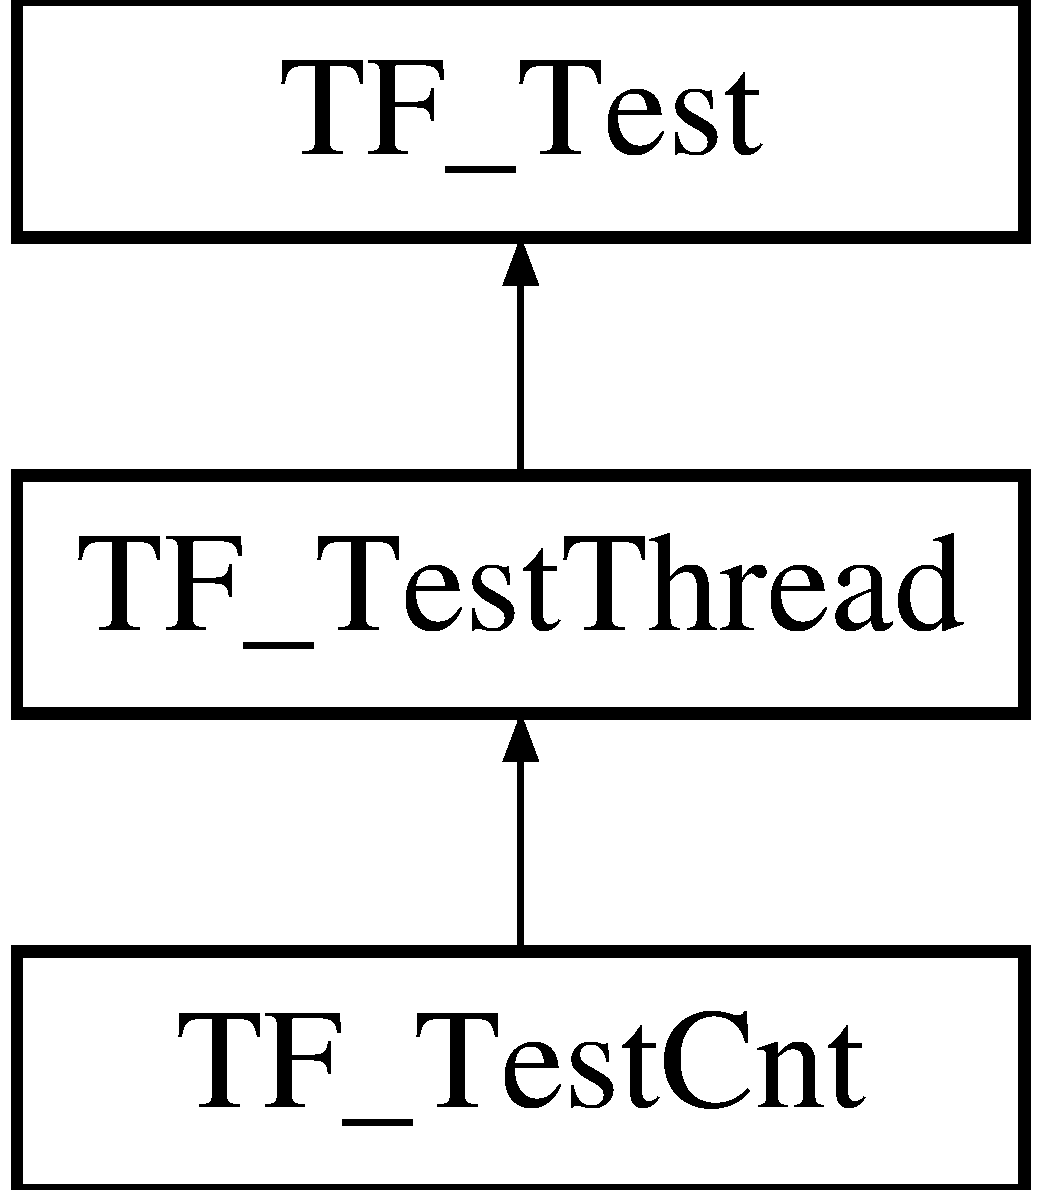
\includegraphics[height=3cm]{classTF__Test}
\end{center}
\end{figure}
\subsection*{Public Member Functions}
\begin{DoxyCompactItemize}
\item 
virtual int \hyperlink{classTF__Test_a26630dcec87c80cd27ab33e3791fbe19}{Prepare} (int cnt)=0
\item 
virtual void \hyperlink{classTF__Test_aab4a87d980709f2756d440771b4e24ac}{Start} (void)=0
\item 
virtual void \hyperlink{classTF__Test_a710a0463dee6767fcb3a3e3d191978b7}{Stop} (void)
\item 
virtual int \hyperlink{classTF__Test_a14768dc0dba16b2cb7be89e8e7c2b3b0}{isComplete} (void)
\item 
virtual void \hyperlink{classTF__Test_ac27a7742873ed7afab48b540fe3d9215}{StepTable} (void)
\item 
virtual void \hyperlink{classTF__Test_a3e4bb4453e490c2a897ccc86b6e788bf}{GetResult} (void)
\end{DoxyCompactItemize}


\subsection{Detailed Description}
Base class for testing device. 

Definition at line 15 of file tf\_\-test.h.

\subsection{Member Function Documentation}
\hypertarget{classTF__Test_a3e4bb4453e490c2a897ccc86b6e788bf}{
\index{TF\_\-Test@{TF\_\-Test}!GetResult@{GetResult}}
\index{GetResult@{GetResult}!TF_Test@{TF\_\-Test}}
\subsubsection[{GetResult}]{\setlength{\rightskip}{0pt plus 5cm}virtual void TF\_\-Test::GetResult (void)\hspace{0.3cm}{\ttfamily  \mbox{[}inline, virtual\mbox{]}}}}
\label{classTF__Test_a3e4bb4453e490c2a897ccc86b6e788bf}


Reimplemented in \hyperlink{classTF__TestCnt_af1d8c610c3b708401c19ad8256db27be}{TF\_\-TestCnt}.

Definition at line 30 of file tf\_\-test.h.\hypertarget{classTF__Test_a14768dc0dba16b2cb7be89e8e7c2b3b0}{
\index{TF\_\-Test@{TF\_\-Test}!isComplete@{isComplete}}
\index{isComplete@{isComplete}!TF_Test@{TF\_\-Test}}
\subsubsection[{isComplete}]{\setlength{\rightskip}{0pt plus 5cm}virtual int TF\_\-Test::isComplete (void)\hspace{0.3cm}{\ttfamily  \mbox{[}inline, virtual\mbox{]}}}}
\label{classTF__Test_a14768dc0dba16b2cb7be89e8e7c2b3b0}


Reimplemented in \hyperlink{classTF__TestThread_a323fe5eecb67f390ee0fada90ade5ed2}{TF\_\-TestThread}.

Definition at line 26 of file tf\_\-test.h.\hypertarget{classTF__Test_a26630dcec87c80cd27ab33e3791fbe19}{
\index{TF\_\-Test@{TF\_\-Test}!Prepare@{Prepare}}
\index{Prepare@{Prepare}!TF_Test@{TF\_\-Test}}
\subsubsection[{Prepare}]{\setlength{\rightskip}{0pt plus 5cm}virtual int TF\_\-Test::Prepare (int {\em cnt})\hspace{0.3cm}{\ttfamily  \mbox{[}pure virtual\mbox{]}}}}
\label{classTF__Test_a26630dcec87c80cd27ab33e3791fbe19}


Implemented in \hyperlink{classTF__TestThread_acfc9a31db91472deb811a47c1cf8e20f}{TF\_\-TestThread}.\hypertarget{classTF__Test_aab4a87d980709f2756d440771b4e24ac}{
\index{TF\_\-Test@{TF\_\-Test}!Start@{Start}}
\index{Start@{Start}!TF_Test@{TF\_\-Test}}
\subsubsection[{Start}]{\setlength{\rightskip}{0pt plus 5cm}virtual void TF\_\-Test::Start (void)\hspace{0.3cm}{\ttfamily  \mbox{[}pure virtual\mbox{]}}}}
\label{classTF__Test_aab4a87d980709f2756d440771b4e24ac}


Implemented in \hyperlink{classTF__TestThread_af7457803ef027ae030d7a98363b9e4b9}{TF\_\-TestThread}.\hypertarget{classTF__Test_ac27a7742873ed7afab48b540fe3d9215}{
\index{TF\_\-Test@{TF\_\-Test}!StepTable@{StepTable}}
\index{StepTable@{StepTable}!TF_Test@{TF\_\-Test}}
\subsubsection[{StepTable}]{\setlength{\rightskip}{0pt plus 5cm}virtual void TF\_\-Test::StepTable (void)\hspace{0.3cm}{\ttfamily  \mbox{[}inline, virtual\mbox{]}}}}
\label{classTF__Test_ac27a7742873ed7afab48b540fe3d9215}


Reimplemented in \hyperlink{classTF__TestCnt_ac1a136199115958172e96ef4c9212351}{TF\_\-TestCnt}, and \hyperlink{classTF__TestThread_a25569ec704c682eed81abd63e05adf2a}{TF\_\-TestThread}.

Definition at line 28 of file tf\_\-test.h.\hypertarget{classTF__Test_a710a0463dee6767fcb3a3e3d191978b7}{
\index{TF\_\-Test@{TF\_\-Test}!Stop@{Stop}}
\index{Stop@{Stop}!TF_Test@{TF\_\-Test}}
\subsubsection[{Stop}]{\setlength{\rightskip}{0pt plus 5cm}virtual void TF\_\-Test::Stop (void)\hspace{0.3cm}{\ttfamily  \mbox{[}inline, virtual\mbox{]}}}}
\label{classTF__Test_a710a0463dee6767fcb3a3e3d191978b7}


Reimplemented in \hyperlink{classTF__TestThread_a3a633a8999b704e85bb197b5fdd63b43}{TF\_\-TestThread}.

Definition at line 24 of file tf\_\-test.h.

The documentation for this class was generated from the following file:\begin{DoxyCompactItemize}
\item 
host/\hyperlink{tf__test_8h}{tf\_\-test.h}\end{DoxyCompactItemize}

\hypertarget{classTF__TestCnt}{
\section{TF\_\-TestCnt Class Reference}
\label{classTF__TestCnt}\index{TF\_\-TestCnt@{TF\_\-TestCnt}}
}


Checking the transmission counter at CUDA device.  


{\ttfamily \#include $<$tf\_\-testcnt.h$>$}Inheritance diagram for TF\_\-TestCnt::\begin{figure}[H]
\begin{center}
\leavevmode
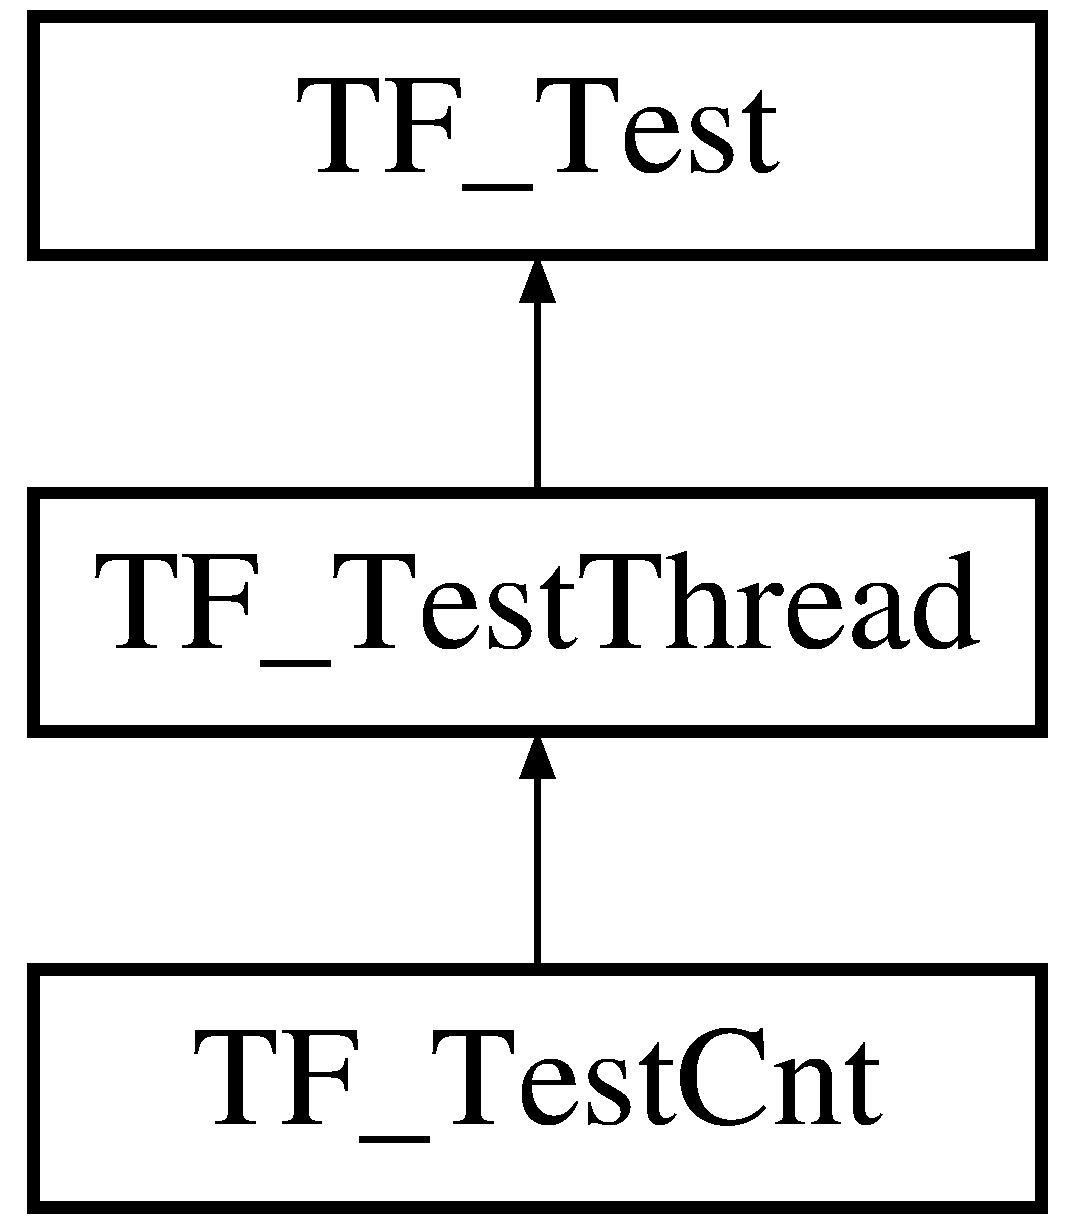
\includegraphics[height=3cm]{classTF__TestCnt}
\end{center}
\end{figure}
\subsection*{Public Member Functions}
\begin{DoxyCompactItemize}
\item 
\hyperlink{classTF__TestCnt_a383dec3bead32626029801edceb9e73d}{TF\_\-TestCnt} (int argc, char $\ast$$\ast$argv)
\item 
virtual \hyperlink{classTF__TestCnt_a05aac39696c9db049193b3a49a389521}{$\sim$TF\_\-TestCnt} ()
\item 
virtual void \hyperlink{classTF__TestCnt_ac1a136199115958172e96ef4c9212351}{StepTable} (void)
\begin{DoxyCompactList}\small\item\em Display current information about cheking buffers. \item\end{DoxyCompactList}\item 
virtual void \hyperlink{classTF__TestCnt_a294a67b58d75600172433b8fae006a3e}{PrepareInThread} (void)
\begin{DoxyCompactList}\small\item\em Prepare CUDA and buffers. \item\end{DoxyCompactList}\item 
virtual void \hyperlink{classTF__TestCnt_a95c7a76a1fe574d1ed260a07f9469501}{CleanupInThread} (void)
\begin{DoxyCompactList}\small\item\em Free buffers and close device. \item\end{DoxyCompactList}\item 
virtual void \hyperlink{classTF__TestCnt_aa7b667d47ddc70942ff2ff73074c7696}{Run} (void)
\begin{DoxyCompactList}\small\item\em Main working cycle. \item\end{DoxyCompactList}\item 
virtual void \hyperlink{classTF__TestCnt_af1d8c610c3b708401c19ad8256db27be}{GetResult} (void)
\begin{DoxyCompactList}\small\item\em Display result for all buffers. \item\end{DoxyCompactList}\item 
void \hyperlink{classTF__TestCnt_adda7871a49f18d707228c85d7169c1df}{FillCounter} (\hyperlink{structCL__Cuda_1_1BAR1__BUF}{CL\_\-Cuda::BAR1\_\-BUF} $\ast$pBar1)
\begin{DoxyCompactList}\small\item\em Fill buffer in Cuda memory via BAR1. \item\end{DoxyCompactList}\item 
void \hyperlink{classTF__TestCnt_a865cbf57a7dcbf45e6ed2a29aac1526c}{GetResultBuffer} (int nbuf)
\begin{DoxyCompactList}\small\item\em Print results for buffer. \item\end{DoxyCompactList}\end{DoxyCompactItemize}
\subsection*{Public Attributes}
\begin{DoxyCompactItemize}
\item 
int \hyperlink{classTF__TestCnt_ae5c1457ee61a41a35a721fcd064892cb}{m\_\-argc}
\begin{DoxyCompactList}\small\item\em Number of arguments. \item\end{DoxyCompactList}\item 
char $\ast$$\ast$ \hyperlink{classTF__TestCnt_a488e38fc6a844dbbf7ec8304717524ef}{m\_\-argv}
\begin{DoxyCompactList}\small\item\em Pointers to arguments. \item\end{DoxyCompactList}\item 
int \hyperlink{classTF__TestCnt_acbae8197757e11371fde750b576e06cc}{m\_\-SizeBufferOfKb}
\begin{DoxyCompactList}\small\item\em Size buffer \mbox{[}kbytes\mbox{]}. Must be n$\ast$64. \item\end{DoxyCompactList}\item 
int \hyperlink{classTF__TestCnt_a70e774fb6d9ae7612e09435db2c181bf}{m\_\-CountOfCycle}
\begin{DoxyCompactList}\small\item\em Number of cycle. 0 -\/ infinitely. \item\end{DoxyCompactList}\item 
struct \hyperlink{structTaskData}{TaskData} $\ast$ \hyperlink{classTF__TestCnt_ad07a631fa0915ea387e2877bf06ef7b2}{td}
\begin{DoxyCompactList}\small\item\em Local data for test. \item\end{DoxyCompactList}\item 
\hyperlink{classCL__Cuda}{CL\_\-Cuda} $\ast$ \hyperlink{classTF__TestCnt_ae3ae3864214526738718e0c7c81e915f}{m\_\-pCuda}
\begin{DoxyCompactList}\small\item\em Cuda device. \item\end{DoxyCompactList}\end{DoxyCompactItemize}


\subsection{Detailed Description}
Checking the transmission counter at CUDA device. Key actions:
\begin{DoxyEnumerate}
\item Open CUDA device
\item Open gpumem driver
\item Allocate three buffers in the CUDA memory
\item Mapping buffers in the BAR1 space on CUDA device
\item Filling the buffer 64-\/bit counter via BAR1
\item Checking buffer in the CUDA device
\item Decimation buffer and transfer to the HOST
\item Transfer result of checking to HOST
\end{DoxyEnumerate}

Steps 5-\/8 are carried out in a loop 

Definition at line 40 of file tf\_\-testcnt.h.

\subsection{Constructor \& Destructor Documentation}
\hypertarget{classTF__TestCnt_a383dec3bead32626029801edceb9e73d}{
\index{TF\_\-TestCnt@{TF\_\-TestCnt}!TF\_\-TestCnt@{TF\_\-TestCnt}}
\index{TF\_\-TestCnt@{TF\_\-TestCnt}!TF_TestCnt@{TF\_\-TestCnt}}
\subsubsection[{TF\_\-TestCnt}]{\setlength{\rightskip}{0pt plus 5cm}TF\_\-TestCnt::TF\_\-TestCnt (int {\em argc}, \/  char $\ast$$\ast$ {\em argv})}}
\label{classTF__TestCnt_a383dec3bead32626029801edceb9e73d}


Definition at line 25 of file tf\_\-testcnt.cpp.\hypertarget{classTF__TestCnt_a05aac39696c9db049193b3a49a389521}{
\index{TF\_\-TestCnt@{TF\_\-TestCnt}!$\sim$TF\_\-TestCnt@{$\sim$TF\_\-TestCnt}}
\index{$\sim$TF\_\-TestCnt@{$\sim$TF\_\-TestCnt}!TF_TestCnt@{TF\_\-TestCnt}}
\subsubsection[{$\sim$TF\_\-TestCnt}]{\setlength{\rightskip}{0pt plus 5cm}TF\_\-TestCnt::$\sim$TF\_\-TestCnt ()\hspace{0.3cm}{\ttfamily  \mbox{[}virtual\mbox{]}}}}
\label{classTF__TestCnt_a05aac39696c9db049193b3a49a389521}


Definition at line 44 of file tf\_\-testcnt.cpp.

\subsection{Member Function Documentation}
\hypertarget{classTF__TestCnt_a95c7a76a1fe574d1ed260a07f9469501}{
\index{TF\_\-TestCnt@{TF\_\-TestCnt}!CleanupInThread@{CleanupInThread}}
\index{CleanupInThread@{CleanupInThread}!TF_TestCnt@{TF\_\-TestCnt}}
\subsubsection[{CleanupInThread}]{\setlength{\rightskip}{0pt plus 5cm}void TF\_\-TestCnt::CleanupInThread (void)\hspace{0.3cm}{\ttfamily  \mbox{[}virtual\mbox{]}}}}
\label{classTF__TestCnt_a95c7a76a1fe574d1ed260a07f9469501}


Free buffers and close device. 

Reimplemented from \hyperlink{classTF__TestThread_a36cfb1a6da55b938b5634ac86adbae2f}{TF\_\-TestThread}.

Definition at line 141 of file tf\_\-testcnt.cpp.\hypertarget{classTF__TestCnt_adda7871a49f18d707228c85d7169c1df}{
\index{TF\_\-TestCnt@{TF\_\-TestCnt}!FillCounter@{FillCounter}}
\index{FillCounter@{FillCounter}!TF_TestCnt@{TF\_\-TestCnt}}
\subsubsection[{FillCounter}]{\setlength{\rightskip}{0pt plus 5cm}void TF\_\-TestCnt::FillCounter ({\bf CL\_\-Cuda::BAR1\_\-BUF} $\ast$ {\em pBar1})}}
\label{classTF__TestCnt_adda7871a49f18d707228c85d7169c1df}


Fill buffer in Cuda memory via BAR1. fill buffer


\begin{DoxyParams}{Parameters}
\item[{\em pBar1}]description of buffer\end{DoxyParams}
function fill bar1 buffer via pBar1-\/$>$app\_\-addr\mbox{[}\mbox{]} 

Definition at line 163 of file tf\_\-testcnt.cpp.\hypertarget{classTF__TestCnt_af1d8c610c3b708401c19ad8256db27be}{
\index{TF\_\-TestCnt@{TF\_\-TestCnt}!GetResult@{GetResult}}
\index{GetResult@{GetResult}!TF_TestCnt@{TF\_\-TestCnt}}
\subsubsection[{GetResult}]{\setlength{\rightskip}{0pt plus 5cm}void TF\_\-TestCnt::GetResult (void)\hspace{0.3cm}{\ttfamily  \mbox{[}virtual\mbox{]}}}}
\label{classTF__TestCnt_af1d8c610c3b708401c19ad8256db27be}


Display result for all buffers. 

Reimplemented from \hyperlink{classTF__Test_a3e4bb4453e490c2a897ccc86b6e788bf}{TF\_\-Test}.

Definition at line 287 of file tf\_\-testcnt.cpp.\hypertarget{classTF__TestCnt_a865cbf57a7dcbf45e6ed2a29aac1526c}{
\index{TF\_\-TestCnt@{TF\_\-TestCnt}!GetResultBuffer@{GetResultBuffer}}
\index{GetResultBuffer@{GetResultBuffer}!TF_TestCnt@{TF\_\-TestCnt}}
\subsubsection[{GetResultBuffer}]{\setlength{\rightskip}{0pt plus 5cm}void TF\_\-TestCnt::GetResultBuffer (int {\em nbuf})}}
\label{classTF__TestCnt_a865cbf57a7dcbf45e6ed2a29aac1526c}


Print results for buffer. Display result for one buffers.


\begin{DoxyParams}{Parameters}
\item[{\em nbuf}]number of buffer \end{DoxyParams}


Definition at line 301 of file tf\_\-testcnt.cpp.\hypertarget{classTF__TestCnt_a294a67b58d75600172433b8fae006a3e}{
\index{TF\_\-TestCnt@{TF\_\-TestCnt}!PrepareInThread@{PrepareInThread}}
\index{PrepareInThread@{PrepareInThread}!TF_TestCnt@{TF\_\-TestCnt}}
\subsubsection[{PrepareInThread}]{\setlength{\rightskip}{0pt plus 5cm}void TF\_\-TestCnt::PrepareInThread (void)\hspace{0.3cm}{\ttfamily  \mbox{[}virtual\mbox{]}}}}
\label{classTF__TestCnt_a294a67b58d75600172433b8fae006a3e}


Prepare CUDA and buffers. Open CUDA device Allocate three buffers and buffer for monitor 

Reimplemented from \hyperlink{classTF__TestThread_aebd5daf255a209019d018bc363021433}{TF\_\-TestThread}.

Definition at line 85 of file tf\_\-testcnt.cpp.\hypertarget{classTF__TestCnt_aa7b667d47ddc70942ff2ff73074c7696}{
\index{TF\_\-TestCnt@{TF\_\-TestCnt}!Run@{Run}}
\index{Run@{Run}!TF_TestCnt@{TF\_\-TestCnt}}
\subsubsection[{Run}]{\setlength{\rightskip}{0pt plus 5cm}void TF\_\-TestCnt::Run (void)\hspace{0.3cm}{\ttfamily  \mbox{[}virtual\mbox{]}}}}
\label{classTF__TestCnt_aa7b667d47ddc70942ff2ff73074c7696}


Main working cycle. It is main working cycle. Function FillCounter simulate to work external DMA channel. 

Reimplemented from \hyperlink{classTF__TestThread_ab581c9fb725595dff5ffc400a96886a0}{TF\_\-TestThread}.

Definition at line 193 of file tf\_\-testcnt.cpp.\hypertarget{classTF__TestCnt_ac1a136199115958172e96ef4c9212351}{
\index{TF\_\-TestCnt@{TF\_\-TestCnt}!StepTable@{StepTable}}
\index{StepTable@{StepTable}!TF_TestCnt@{TF\_\-TestCnt}}
\subsubsection[{StepTable}]{\setlength{\rightskip}{0pt plus 5cm}void TF\_\-TestCnt::StepTable (void)\hspace{0.3cm}{\ttfamily  \mbox{[}virtual\mbox{]}}}}
\label{classTF__TestCnt_ac1a136199115958172e96ef4c9212351}


Display current information about cheking buffers. Function display information if 0==m\_\-CountOfCycle function is called from main with interval of 100 ms 

Reimplemented from \hyperlink{classTF__TestThread_a25569ec704c682eed81abd63e05adf2a}{TF\_\-TestThread}.

Definition at line 57 of file tf\_\-testcnt.cpp.

\subsection{Member Data Documentation}
\hypertarget{classTF__TestCnt_ae5c1457ee61a41a35a721fcd064892cb}{
\index{TF\_\-TestCnt@{TF\_\-TestCnt}!m\_\-argc@{m\_\-argc}}
\index{m\_\-argc@{m\_\-argc}!TF_TestCnt@{TF\_\-TestCnt}}
\subsubsection[{m\_\-argc}]{\setlength{\rightskip}{0pt plus 5cm}int {\bf TF\_\-TestCnt::m\_\-argc}}}
\label{classTF__TestCnt_ae5c1457ee61a41a35a721fcd064892cb}


Number of arguments. 

Definition at line 58 of file tf\_\-testcnt.h.\hypertarget{classTF__TestCnt_a488e38fc6a844dbbf7ec8304717524ef}{
\index{TF\_\-TestCnt@{TF\_\-TestCnt}!m\_\-argv@{m\_\-argv}}
\index{m\_\-argv@{m\_\-argv}!TF_TestCnt@{TF\_\-TestCnt}}
\subsubsection[{m\_\-argv}]{\setlength{\rightskip}{0pt plus 5cm}char$\ast$$\ast$ {\bf TF\_\-TestCnt::m\_\-argv}}}
\label{classTF__TestCnt_a488e38fc6a844dbbf7ec8304717524ef}


Pointers to arguments. 

Definition at line 61 of file tf\_\-testcnt.h.\hypertarget{classTF__TestCnt_a70e774fb6d9ae7612e09435db2c181bf}{
\index{TF\_\-TestCnt@{TF\_\-TestCnt}!m\_\-CountOfCycle@{m\_\-CountOfCycle}}
\index{m\_\-CountOfCycle@{m\_\-CountOfCycle}!TF_TestCnt@{TF\_\-TestCnt}}
\subsubsection[{m\_\-CountOfCycle}]{\setlength{\rightskip}{0pt plus 5cm}int {\bf TF\_\-TestCnt::m\_\-CountOfCycle}}}
\label{classTF__TestCnt_a70e774fb6d9ae7612e09435db2c181bf}


Number of cycle. 0 -\/ infinitely. 

Definition at line 66 of file tf\_\-testcnt.h.\hypertarget{classTF__TestCnt_ae3ae3864214526738718e0c7c81e915f}{
\index{TF\_\-TestCnt@{TF\_\-TestCnt}!m\_\-pCuda@{m\_\-pCuda}}
\index{m\_\-pCuda@{m\_\-pCuda}!TF_TestCnt@{TF\_\-TestCnt}}
\subsubsection[{m\_\-pCuda}]{\setlength{\rightskip}{0pt plus 5cm}{\bf CL\_\-Cuda}$\ast$ {\bf TF\_\-TestCnt::m\_\-pCuda}}}
\label{classTF__TestCnt_ae3ae3864214526738718e0c7c81e915f}


Cuda device. 

Definition at line 71 of file tf\_\-testcnt.h.\hypertarget{classTF__TestCnt_acbae8197757e11371fde750b576e06cc}{
\index{TF\_\-TestCnt@{TF\_\-TestCnt}!m\_\-SizeBufferOfKb@{m\_\-SizeBufferOfKb}}
\index{m\_\-SizeBufferOfKb@{m\_\-SizeBufferOfKb}!TF_TestCnt@{TF\_\-TestCnt}}
\subsubsection[{m\_\-SizeBufferOfKb}]{\setlength{\rightskip}{0pt plus 5cm}int {\bf TF\_\-TestCnt::m\_\-SizeBufferOfKb}}}
\label{classTF__TestCnt_acbae8197757e11371fde750b576e06cc}


Size buffer \mbox{[}kbytes\mbox{]}. Must be n$\ast$64. 

Definition at line 64 of file tf\_\-testcnt.h.\hypertarget{classTF__TestCnt_ad07a631fa0915ea387e2877bf06ef7b2}{
\index{TF\_\-TestCnt@{TF\_\-TestCnt}!td@{td}}
\index{td@{td}!TF_TestCnt@{TF\_\-TestCnt}}
\subsubsection[{td}]{\setlength{\rightskip}{0pt plus 5cm}struct {\bf TaskData}$\ast$ {\bf TF\_\-TestCnt::td}\hspace{0.3cm}{\ttfamily  \mbox{[}read\mbox{]}}}}
\label{classTF__TestCnt_ad07a631fa0915ea387e2877bf06ef7b2}


Local data for test. 

Definition at line 69 of file tf\_\-testcnt.h.

The documentation for this class was generated from the following files:\begin{DoxyCompactItemize}
\item 
host/\hyperlink{tf__testcnt_8h}{tf\_\-testcnt.h}\item 
host/\hyperlink{tf__testcnt_8cpp}{tf\_\-testcnt.cpp}\end{DoxyCompactItemize}

\hypertarget{classTF__TestThread}{
\section{TF\_\-TestThread Class Reference}
\label{classTF__TestThread}\index{TF\_\-TestThread@{TF\_\-TestThread}}
}


Base class for application with thread.  


{\ttfamily \#include $<$tf\_\-testthread.h$>$}Inheritance diagram for TF\_\-TestThread::\begin{figure}[H]
\begin{center}
\leavevmode
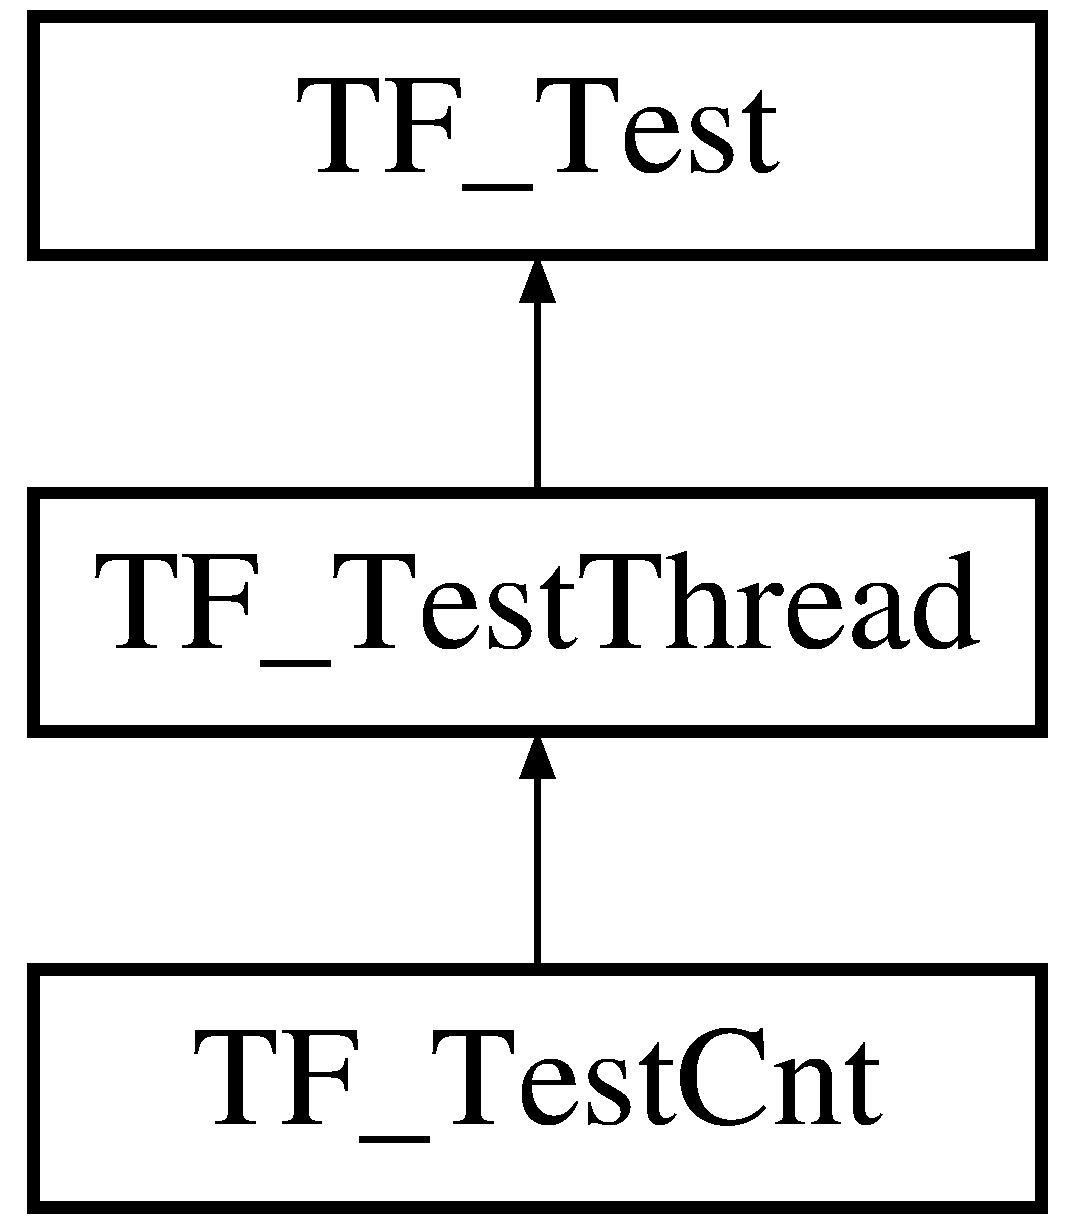
\includegraphics[height=3cm]{classTF__TestThread}
\end{center}
\end{figure}
\subsection*{Public Member Functions}
\begin{DoxyCompactItemize}
\item 
\hyperlink{classTF__TestThread_adc0b50667619b13b3791f96f8d9f3f9e}{TF\_\-TestThread} (int argc, char $\ast$$\ast$argv)
\item 
virtual \hyperlink{classTF__TestThread_a98193a8f032be71f6722230a528cb497}{$\sim$TF\_\-TestThread} ()
\item 
virtual int \hyperlink{classTF__TestThread_acfc9a31db91472deb811a47c1cf8e20f}{Prepare} (int cnt)
\item 
virtual void \hyperlink{classTF__TestThread_af7457803ef027ae030d7a98363b9e4b9}{Start} (void)
\item 
virtual void \hyperlink{classTF__TestThread_a3a633a8999b704e85bb197b5fdd63b43}{Stop} (void)
\item 
virtual int \hyperlink{classTF__TestThread_a323fe5eecb67f390ee0fada90ade5ed2}{isComplete} (void)
\item 
virtual void \hyperlink{classTF__TestThread_a25569ec704c682eed81abd63e05adf2a}{StepTable} (void)
\item 
void $\ast$ \hyperlink{classTF__TestThread_aac0ee4d59a3fa57e93ad2fa33644b377}{Execute} (void)
\item 
virtual void \hyperlink{classTF__TestThread_aebd5daf255a209019d018bc363021433}{PrepareInThread} (void)
\item 
virtual void \hyperlink{classTF__TestThread_a36cfb1a6da55b938b5634ac86adbae2f}{CleanupInThread} (void)
\item 
virtual void \hyperlink{classTF__TestThread_ab581c9fb725595dff5ffc400a96886a0}{Run} (void)
\item 
int \hyperlink{classTF__TestThread_a3cd8bd0134a8c180c885e7fb19cc9b3c}{GetFromCommnadLine} (int argc, char $\ast$$\ast$argv, char $\ast$name, int defValue)
\begin{DoxyCompactList}\small\item\em get value from command line \item\end{DoxyCompactList}\end{DoxyCompactItemize}
\subsection*{Static Public Member Functions}
\begin{DoxyCompactItemize}
\item 
static void $\ast$ \hyperlink{classTF__TestThread_a9ba6692148ce51f4bbfff8f408479c1f}{ThreadFunc} (void $\ast$lpvThreadParm)
\end{DoxyCompactItemize}
\subsection*{Public Attributes}
\begin{DoxyCompactItemize}
\item 
int \hyperlink{classTF__TestThread_a5d92ac2f7010e79fb40326aa8980ddf3}{m\_\-isPrepareComplete}
\item 
int \hyperlink{classTF__TestThread_ab3f42e170b84b6b124fae56d403504c1}{m\_\-isComplete}
\item 
int \hyperlink{classTF__TestThread_ab7e24e3d4b9d6beb4a49d8845f5b2d9f}{m\_\-isTerminate}
\item 
int \hyperlink{classTF__TestThread_a796b7c7257792b3eabdb65b3e3d8d990}{m\_\-CycleCnt}
\item 
pthread\_\-mutex\_\-t \hyperlink{classTF__TestThread_a1ad6411cf734262c0d8e58a763c88cfb}{m\_\-StartMutex}
\item 
pthread\_\-cond\_\-t \hyperlink{classTF__TestThread_a45462e11e298f01d4868e084aa67be1c}{m\_\-StartCond}
\item 
pthread\_\-t \hyperlink{classTF__TestThread_a0c8b8d93ed2ae109221ea8da813ec389}{m\_\-hThread}
\item 
pthread\_\-attr\_\-t \hyperlink{classTF__TestThread_a111456494b43af46290cccae56efd170}{m\_\-attrThread}
\end{DoxyCompactItemize}


\subsection{Detailed Description}
Base class for application with thread. 

Definition at line 21 of file tf\_\-testthread.h.

\subsection{Constructor \& Destructor Documentation}
\hypertarget{classTF__TestThread_adc0b50667619b13b3791f96f8d9f3f9e}{
\index{TF\_\-TestThread@{TF\_\-TestThread}!TF\_\-TestThread@{TF\_\-TestThread}}
\index{TF\_\-TestThread@{TF\_\-TestThread}!TF_TestThread@{TF\_\-TestThread}}
\subsubsection[{TF\_\-TestThread}]{\setlength{\rightskip}{0pt plus 5cm}TF\_\-TestThread::TF\_\-TestThread (int {\em argc}, \/  char $\ast$$\ast$ {\em argv})}}
\label{classTF__TestThread_adc0b50667619b13b3791f96f8d9f3f9e}


Definition at line 18 of file tf\_\-testthread.cpp.\hypertarget{classTF__TestThread_a98193a8f032be71f6722230a528cb497}{
\index{TF\_\-TestThread@{TF\_\-TestThread}!$\sim$TF\_\-TestThread@{$\sim$TF\_\-TestThread}}
\index{$\sim$TF\_\-TestThread@{$\sim$TF\_\-TestThread}!TF_TestThread@{TF\_\-TestThread}}
\subsubsection[{$\sim$TF\_\-TestThread}]{\setlength{\rightskip}{0pt plus 5cm}TF\_\-TestThread::$\sim$TF\_\-TestThread ()\hspace{0.3cm}{\ttfamily  \mbox{[}virtual\mbox{]}}}}
\label{classTF__TestThread_a98193a8f032be71f6722230a528cb497}


Definition at line 32 of file tf\_\-testthread.cpp.

\subsection{Member Function Documentation}
\hypertarget{classTF__TestThread_a36cfb1a6da55b938b5634ac86adbae2f}{
\index{TF\_\-TestThread@{TF\_\-TestThread}!CleanupInThread@{CleanupInThread}}
\index{CleanupInThread@{CleanupInThread}!TF_TestThread@{TF\_\-TestThread}}
\subsubsection[{CleanupInThread}]{\setlength{\rightskip}{0pt plus 5cm}virtual void TF\_\-TestThread::CleanupInThread (void)\hspace{0.3cm}{\ttfamily  \mbox{[}inline, virtual\mbox{]}}}}
\label{classTF__TestThread_a36cfb1a6da55b938b5634ac86adbae2f}


Reimplemented in \hyperlink{classTF__TestCnt_a95c7a76a1fe574d1ed260a07f9469501}{TF\_\-TestCnt}.

Definition at line 44 of file tf\_\-testthread.h.\hypertarget{classTF__TestThread_aac0ee4d59a3fa57e93ad2fa33644b377}{
\index{TF\_\-TestThread@{TF\_\-TestThread}!Execute@{Execute}}
\index{Execute@{Execute}!TF_TestThread@{TF\_\-TestThread}}
\subsubsection[{Execute}]{\setlength{\rightskip}{0pt plus 5cm}void $\ast$ TF\_\-TestThread::Execute (void)}}
\label{classTF__TestThread_aac0ee4d59a3fa57e93ad2fa33644b377}


Definition at line 77 of file tf\_\-testthread.cpp.\hypertarget{classTF__TestThread_a3cd8bd0134a8c180c885e7fb19cc9b3c}{
\index{TF\_\-TestThread@{TF\_\-TestThread}!GetFromCommnadLine@{GetFromCommnadLine}}
\index{GetFromCommnadLine@{GetFromCommnadLine}!TF_TestThread@{TF\_\-TestThread}}
\subsubsection[{GetFromCommnadLine}]{\setlength{\rightskip}{0pt plus 5cm}int TF\_\-TestThread::GetFromCommnadLine (int {\em argc}, \/  char $\ast$$\ast$ {\em argv}, \/  char $\ast$ {\em name}, \/  int {\em defValue})}}
\label{classTF__TestThread_a3cd8bd0134a8c180c885e7fb19cc9b3c}


get value from command line format command line: $<$name1$>$ $<$value1$>$ $<$name2$>$ $<$value2$>$


\begin{DoxyParams}{Parameters}
\item[{\em argc}]number of argument \item[{\em argv}]pointers to arguments \item[{\em name}]key of argument  defValue default value for arguments\end{DoxyParams}
\begin{DoxyReturn}{Returns}
value of argument or default value of argument 
\end{DoxyReturn}


Definition at line 128 of file tf\_\-testthread.cpp.\hypertarget{classTF__TestThread_a323fe5eecb67f390ee0fada90ade5ed2}{
\index{TF\_\-TestThread@{TF\_\-TestThread}!isComplete@{isComplete}}
\index{isComplete@{isComplete}!TF_TestThread@{TF\_\-TestThread}}
\subsubsection[{isComplete}]{\setlength{\rightskip}{0pt plus 5cm}int TF\_\-TestThread::isComplete (void)\hspace{0.3cm}{\ttfamily  \mbox{[}virtual\mbox{]}}}}
\label{classTF__TestThread_a323fe5eecb67f390ee0fada90ade5ed2}


Reimplemented from \hyperlink{classTF__Test_a14768dc0dba16b2cb7be89e8e7c2b3b0}{TF\_\-Test}.

Definition at line 110 of file tf\_\-testthread.cpp.\hypertarget{classTF__TestThread_acfc9a31db91472deb811a47c1cf8e20f}{
\index{TF\_\-TestThread@{TF\_\-TestThread}!Prepare@{Prepare}}
\index{Prepare@{Prepare}!TF_TestThread@{TF\_\-TestThread}}
\subsubsection[{Prepare}]{\setlength{\rightskip}{0pt plus 5cm}int TF\_\-TestThread::Prepare (int {\em cnt})\hspace{0.3cm}{\ttfamily  \mbox{[}virtual\mbox{]}}}}
\label{classTF__TestThread_acfc9a31db91472deb811a47c1cf8e20f}


Implements \hyperlink{classTF__Test_a26630dcec87c80cd27ab33e3791fbe19}{TF\_\-Test}.

Definition at line 39 of file tf\_\-testthread.cpp.\hypertarget{classTF__TestThread_aebd5daf255a209019d018bc363021433}{
\index{TF\_\-TestThread@{TF\_\-TestThread}!PrepareInThread@{PrepareInThread}}
\index{PrepareInThread@{PrepareInThread}!TF_TestThread@{TF\_\-TestThread}}
\subsubsection[{PrepareInThread}]{\setlength{\rightskip}{0pt plus 5cm}virtual void TF\_\-TestThread::PrepareInThread (void)\hspace{0.3cm}{\ttfamily  \mbox{[}inline, virtual\mbox{]}}}}
\label{classTF__TestThread_aebd5daf255a209019d018bc363021433}


Reimplemented in \hyperlink{classTF__TestCnt_a294a67b58d75600172433b8fae006a3e}{TF\_\-TestCnt}.

Definition at line 42 of file tf\_\-testthread.h.\hypertarget{classTF__TestThread_ab581c9fb725595dff5ffc400a96886a0}{
\index{TF\_\-TestThread@{TF\_\-TestThread}!Run@{Run}}
\index{Run@{Run}!TF_TestThread@{TF\_\-TestThread}}
\subsubsection[{Run}]{\setlength{\rightskip}{0pt plus 5cm}virtual void TF\_\-TestThread::Run (void)\hspace{0.3cm}{\ttfamily  \mbox{[}inline, virtual\mbox{]}}}}
\label{classTF__TestThread_ab581c9fb725595dff5ffc400a96886a0}


Reimplemented in \hyperlink{classTF__TestCnt_aa7b667d47ddc70942ff2ff73074c7696}{TF\_\-TestCnt}.

Definition at line 46 of file tf\_\-testthread.h.\hypertarget{classTF__TestThread_af7457803ef027ae030d7a98363b9e4b9}{
\index{TF\_\-TestThread@{TF\_\-TestThread}!Start@{Start}}
\index{Start@{Start}!TF_TestThread@{TF\_\-TestThread}}
\subsubsection[{Start}]{\setlength{\rightskip}{0pt plus 5cm}void TF\_\-TestThread::Start (void)\hspace{0.3cm}{\ttfamily  \mbox{[}virtual\mbox{]}}}}
\label{classTF__TestThread_af7457803ef027ae030d7a98363b9e4b9}


Implements \hyperlink{classTF__Test_aab4a87d980709f2756d440771b4e24ac}{TF\_\-Test}.

Definition at line 95 of file tf\_\-testthread.cpp.\hypertarget{classTF__TestThread_a25569ec704c682eed81abd63e05adf2a}{
\index{TF\_\-TestThread@{TF\_\-TestThread}!StepTable@{StepTable}}
\index{StepTable@{StepTable}!TF_TestThread@{TF\_\-TestThread}}
\subsubsection[{StepTable}]{\setlength{\rightskip}{0pt plus 5cm}virtual void TF\_\-TestThread::StepTable (void)\hspace{0.3cm}{\ttfamily  \mbox{[}inline, virtual\mbox{]}}}}
\label{classTF__TestThread_a25569ec704c682eed81abd63e05adf2a}


Reimplemented from \hyperlink{classTF__Test_ac27a7742873ed7afab48b540fe3d9215}{TF\_\-Test}.

Reimplemented in \hyperlink{classTF__TestCnt_ac1a136199115958172e96ef4c9212351}{TF\_\-TestCnt}.

Definition at line 35 of file tf\_\-testthread.h.\hypertarget{classTF__TestThread_a3a633a8999b704e85bb197b5fdd63b43}{
\index{TF\_\-TestThread@{TF\_\-TestThread}!Stop@{Stop}}
\index{Stop@{Stop}!TF_TestThread@{TF\_\-TestThread}}
\subsubsection[{Stop}]{\setlength{\rightskip}{0pt plus 5cm}void TF\_\-TestThread::Stop (void)\hspace{0.3cm}{\ttfamily  \mbox{[}virtual\mbox{]}}}}
\label{classTF__TestThread_a3a633a8999b704e85bb197b5fdd63b43}


Reimplemented from \hyperlink{classTF__Test_a710a0463dee6767fcb3a3e3d191978b7}{TF\_\-Test}.

Definition at line 104 of file tf\_\-testthread.cpp.\hypertarget{classTF__TestThread_a9ba6692148ce51f4bbfff8f408479c1f}{
\index{TF\_\-TestThread@{TF\_\-TestThread}!ThreadFunc@{ThreadFunc}}
\index{ThreadFunc@{ThreadFunc}!TF_TestThread@{TF\_\-TestThread}}
\subsubsection[{ThreadFunc}]{\setlength{\rightskip}{0pt plus 5cm}void $\ast$ TF\_\-TestThread::ThreadFunc (void $\ast$ {\em lpvThreadParm})\hspace{0.3cm}{\ttfamily  \mbox{[}static\mbox{]}}}}
\label{classTF__TestThread_a9ba6692148ce51f4bbfff8f408479c1f}


Definition at line 67 of file tf\_\-testthread.cpp.

\subsection{Member Data Documentation}
\hypertarget{classTF__TestThread_a111456494b43af46290cccae56efd170}{
\index{TF\_\-TestThread@{TF\_\-TestThread}!m\_\-attrThread@{m\_\-attrThread}}
\index{m\_\-attrThread@{m\_\-attrThread}!TF_TestThread@{TF\_\-TestThread}}
\subsubsection[{m\_\-attrThread}]{\setlength{\rightskip}{0pt plus 5cm}pthread\_\-attr\_\-t {\bf TF\_\-TestThread::m\_\-attrThread}}}
\label{classTF__TestThread_a111456494b43af46290cccae56efd170}


Definition at line 59 of file tf\_\-testthread.h.\hypertarget{classTF__TestThread_a796b7c7257792b3eabdb65b3e3d8d990}{
\index{TF\_\-TestThread@{TF\_\-TestThread}!m\_\-CycleCnt@{m\_\-CycleCnt}}
\index{m\_\-CycleCnt@{m\_\-CycleCnt}!TF_TestThread@{TF\_\-TestThread}}
\subsubsection[{m\_\-CycleCnt}]{\setlength{\rightskip}{0pt plus 5cm}int {\bf TF\_\-TestThread::m\_\-CycleCnt}}}
\label{classTF__TestThread_a796b7c7257792b3eabdb65b3e3d8d990}


Definition at line 53 of file tf\_\-testthread.h.\hypertarget{classTF__TestThread_a0c8b8d93ed2ae109221ea8da813ec389}{
\index{TF\_\-TestThread@{TF\_\-TestThread}!m\_\-hThread@{m\_\-hThread}}
\index{m\_\-hThread@{m\_\-hThread}!TF_TestThread@{TF\_\-TestThread}}
\subsubsection[{m\_\-hThread}]{\setlength{\rightskip}{0pt plus 5cm}pthread\_\-t {\bf TF\_\-TestThread::m\_\-hThread}}}
\label{classTF__TestThread_a0c8b8d93ed2ae109221ea8da813ec389}


Definition at line 58 of file tf\_\-testthread.h.\hypertarget{classTF__TestThread_ab3f42e170b84b6b124fae56d403504c1}{
\index{TF\_\-TestThread@{TF\_\-TestThread}!m\_\-isComplete@{m\_\-isComplete}}
\index{m\_\-isComplete@{m\_\-isComplete}!TF_TestThread@{TF\_\-TestThread}}
\subsubsection[{m\_\-isComplete}]{\setlength{\rightskip}{0pt plus 5cm}int {\bf TF\_\-TestThread::m\_\-isComplete}}}
\label{classTF__TestThread_ab3f42e170b84b6b124fae56d403504c1}


Definition at line 50 of file tf\_\-testthread.h.\hypertarget{classTF__TestThread_a5d92ac2f7010e79fb40326aa8980ddf3}{
\index{TF\_\-TestThread@{TF\_\-TestThread}!m\_\-isPrepareComplete@{m\_\-isPrepareComplete}}
\index{m\_\-isPrepareComplete@{m\_\-isPrepareComplete}!TF_TestThread@{TF\_\-TestThread}}
\subsubsection[{m\_\-isPrepareComplete}]{\setlength{\rightskip}{0pt plus 5cm}int {\bf TF\_\-TestThread::m\_\-isPrepareComplete}}}
\label{classTF__TestThread_a5d92ac2f7010e79fb40326aa8980ddf3}


Definition at line 46 of file tf\_\-testthread.h.\hypertarget{classTF__TestThread_ab7e24e3d4b9d6beb4a49d8845f5b2d9f}{
\index{TF\_\-TestThread@{TF\_\-TestThread}!m\_\-isTerminate@{m\_\-isTerminate}}
\index{m\_\-isTerminate@{m\_\-isTerminate}!TF_TestThread@{TF\_\-TestThread}}
\subsubsection[{m\_\-isTerminate}]{\setlength{\rightskip}{0pt plus 5cm}int {\bf TF\_\-TestThread::m\_\-isTerminate}}}
\label{classTF__TestThread_ab7e24e3d4b9d6beb4a49d8845f5b2d9f}


Definition at line 51 of file tf\_\-testthread.h.\hypertarget{classTF__TestThread_a45462e11e298f01d4868e084aa67be1c}{
\index{TF\_\-TestThread@{TF\_\-TestThread}!m\_\-StartCond@{m\_\-StartCond}}
\index{m\_\-StartCond@{m\_\-StartCond}!TF_TestThread@{TF\_\-TestThread}}
\subsubsection[{m\_\-StartCond}]{\setlength{\rightskip}{0pt plus 5cm}pthread\_\-cond\_\-t {\bf TF\_\-TestThread::m\_\-StartCond}}}
\label{classTF__TestThread_a45462e11e298f01d4868e084aa67be1c}


Definition at line 56 of file tf\_\-testthread.h.\hypertarget{classTF__TestThread_a1ad6411cf734262c0d8e58a763c88cfb}{
\index{TF\_\-TestThread@{TF\_\-TestThread}!m\_\-StartMutex@{m\_\-StartMutex}}
\index{m\_\-StartMutex@{m\_\-StartMutex}!TF_TestThread@{TF\_\-TestThread}}
\subsubsection[{m\_\-StartMutex}]{\setlength{\rightskip}{0pt plus 5cm}pthread\_\-mutex\_\-t {\bf TF\_\-TestThread::m\_\-StartMutex}}}
\label{classTF__TestThread_a1ad6411cf734262c0d8e58a763c88cfb}


Definition at line 55 of file tf\_\-testthread.h.

The documentation for this class was generated from the following files:\begin{DoxyCompactItemize}
\item 
host/\hyperlink{tf__testthread_8h}{tf\_\-testthread.h}\item 
host/\hyperlink{tf__testthread_8cpp}{tf\_\-testthread.cpp}\end{DoxyCompactItemize}

\chapter{File Documentation}
\hypertarget{gpumemioctl_8h}{
\section{common/gpumemioctl.h File Reference}
\label{gpumemioctl_8h}\index{common/gpumemioctl.h@{common/gpumemioctl.h}}
}
\subsection*{Classes}
\begin{DoxyCompactItemize}
\item 
struct \hyperlink{structgpudma__lock__t}{gpudma\_\-lock\_\-t}
\item 
struct \hyperlink{structgpudma__unlock__t}{gpudma\_\-unlock\_\-t}
\item 
struct \hyperlink{structgpudma__state__t}{gpudma\_\-state\_\-t}
\end{DoxyCompactItemize}
\subsection*{Defines}
\begin{DoxyCompactItemize}
\item 
\#define \hyperlink{gpumemioctl_8h_a68ca8a3c618bdad437c63e5c11d8258c}{GPUMEM\_\-DRIVER\_\-NAME}~\char`\"{}gpumem\char`\"{}
\item 
\#define \hyperlink{gpumemioctl_8h_a551e82be9f0d0557ce4832e876908ce2}{IOCTL\_\-GPUMEM\_\-LOCK}~GPUMEM\_\-MAKE\_\-IOCTL(10)
\item 
\#define \hyperlink{gpumemioctl_8h_a692ca08110c03a4a9d420c951f9d3dfb}{IOCTL\_\-GPUMEM\_\-UNLOCK}~GPUMEM\_\-MAKE\_\-IOCTL(11)
\item 
\#define \hyperlink{gpumemioctl_8h_ae81776f1d36b679d1528d091444c8179}{IOCTL\_\-GPUMEM\_\-STATE}~GPUMEM\_\-MAKE\_\-IOCTL(12)
\item 
\#define \hyperlink{gpumemioctl_8h_ab252c9e0bae490c0a817ae0e19b9a631}{GPU\_\-BOUND\_\-SHIFT}~16
\item 
\#define \hyperlink{gpumemioctl_8h_ab22d69043dedd74f41fa107d49bf702b}{GPU\_\-BOUND\_\-SIZE}~((u64)1 $<$$<$ GPU\_\-BOUND\_\-SHIFT)
\item 
\#define \hyperlink{gpumemioctl_8h_a41acdc8f2c8a661059c35518ab48f3ed}{GPU\_\-BOUND\_\-OFFSET}~(GPU\_\-BOUND\_\-SIZE-\/1)
\item 
\#define \hyperlink{gpumemioctl_8h_a6fbe483c510258ee42d147725054677d}{GPU\_\-BOUND\_\-MASK}~($\sim$GPU\_\-BOUND\_\-OFFSET)
\end{DoxyCompactItemize}


\subsection{Define Documentation}
\hypertarget{gpumemioctl_8h_a6fbe483c510258ee42d147725054677d}{
\index{gpumemioctl.h@{gpumemioctl.h}!GPU\_\-BOUND\_\-MASK@{GPU\_\-BOUND\_\-MASK}}
\index{GPU\_\-BOUND\_\-MASK@{GPU\_\-BOUND\_\-MASK}!gpumemioctl.h@{gpumemioctl.h}}
\subsubsection[{GPU\_\-BOUND\_\-MASK}]{\setlength{\rightskip}{0pt plus 5cm}\#define GPU\_\-BOUND\_\-MASK~($\sim$GPU\_\-BOUND\_\-OFFSET)}}
\label{gpumemioctl_8h_a6fbe483c510258ee42d147725054677d}


Definition at line 29 of file gpumemioctl.h.\hypertarget{gpumemioctl_8h_a41acdc8f2c8a661059c35518ab48f3ed}{
\index{gpumemioctl.h@{gpumemioctl.h}!GPU\_\-BOUND\_\-OFFSET@{GPU\_\-BOUND\_\-OFFSET}}
\index{GPU\_\-BOUND\_\-OFFSET@{GPU\_\-BOUND\_\-OFFSET}!gpumemioctl.h@{gpumemioctl.h}}
\subsubsection[{GPU\_\-BOUND\_\-OFFSET}]{\setlength{\rightskip}{0pt plus 5cm}\#define GPU\_\-BOUND\_\-OFFSET~(GPU\_\-BOUND\_\-SIZE-\/1)}}
\label{gpumemioctl_8h_a41acdc8f2c8a661059c35518ab48f3ed}


Definition at line 28 of file gpumemioctl.h.\hypertarget{gpumemioctl_8h_ab252c9e0bae490c0a817ae0e19b9a631}{
\index{gpumemioctl.h@{gpumemioctl.h}!GPU\_\-BOUND\_\-SHIFT@{GPU\_\-BOUND\_\-SHIFT}}
\index{GPU\_\-BOUND\_\-SHIFT@{GPU\_\-BOUND\_\-SHIFT}!gpumemioctl.h@{gpumemioctl.h}}
\subsubsection[{GPU\_\-BOUND\_\-SHIFT}]{\setlength{\rightskip}{0pt plus 5cm}\#define GPU\_\-BOUND\_\-SHIFT~16}}
\label{gpumemioctl_8h_ab252c9e0bae490c0a817ae0e19b9a631}


Definition at line 26 of file gpumemioctl.h.\hypertarget{gpumemioctl_8h_ab22d69043dedd74f41fa107d49bf702b}{
\index{gpumemioctl.h@{gpumemioctl.h}!GPU\_\-BOUND\_\-SIZE@{GPU\_\-BOUND\_\-SIZE}}
\index{GPU\_\-BOUND\_\-SIZE@{GPU\_\-BOUND\_\-SIZE}!gpumemioctl.h@{gpumemioctl.h}}
\subsubsection[{GPU\_\-BOUND\_\-SIZE}]{\setlength{\rightskip}{0pt plus 5cm}\#define GPU\_\-BOUND\_\-SIZE~((u64)1 $<$$<$ GPU\_\-BOUND\_\-SHIFT)}}
\label{gpumemioctl_8h_ab22d69043dedd74f41fa107d49bf702b}


Definition at line 27 of file gpumemioctl.h.\hypertarget{gpumemioctl_8h_a68ca8a3c618bdad437c63e5c11d8258c}{
\index{gpumemioctl.h@{gpumemioctl.h}!GPUMEM\_\-DRIVER\_\-NAME@{GPUMEM\_\-DRIVER\_\-NAME}}
\index{GPUMEM\_\-DRIVER\_\-NAME@{GPUMEM\_\-DRIVER\_\-NAME}!gpumemioctl.h@{gpumemioctl.h}}
\subsubsection[{GPUMEM\_\-DRIVER\_\-NAME}]{\setlength{\rightskip}{0pt plus 5cm}\#define GPUMEM\_\-DRIVER\_\-NAME~\char`\"{}gpumem\char`\"{}}}
\label{gpumemioctl_8h_a68ca8a3c618bdad437c63e5c11d8258c}


Definition at line 7 of file gpumemioctl.h.\hypertarget{gpumemioctl_8h_a551e82be9f0d0557ce4832e876908ce2}{
\index{gpumemioctl.h@{gpumemioctl.h}!IOCTL\_\-GPUMEM\_\-LOCK@{IOCTL\_\-GPUMEM\_\-LOCK}}
\index{IOCTL\_\-GPUMEM\_\-LOCK@{IOCTL\_\-GPUMEM\_\-LOCK}!gpumemioctl.h@{gpumemioctl.h}}
\subsubsection[{IOCTL\_\-GPUMEM\_\-LOCK}]{\setlength{\rightskip}{0pt plus 5cm}\#define IOCTL\_\-GPUMEM\_\-LOCK~GPUMEM\_\-MAKE\_\-IOCTL(10)}}
\label{gpumemioctl_8h_a551e82be9f0d0557ce4832e876908ce2}


Definition at line 20 of file gpumemioctl.h.\hypertarget{gpumemioctl_8h_ae81776f1d36b679d1528d091444c8179}{
\index{gpumemioctl.h@{gpumemioctl.h}!IOCTL\_\-GPUMEM\_\-STATE@{IOCTL\_\-GPUMEM\_\-STATE}}
\index{IOCTL\_\-GPUMEM\_\-STATE@{IOCTL\_\-GPUMEM\_\-STATE}!gpumemioctl.h@{gpumemioctl.h}}
\subsubsection[{IOCTL\_\-GPUMEM\_\-STATE}]{\setlength{\rightskip}{0pt plus 5cm}\#define IOCTL\_\-GPUMEM\_\-STATE~GPUMEM\_\-MAKE\_\-IOCTL(12)}}
\label{gpumemioctl_8h_ae81776f1d36b679d1528d091444c8179}


Definition at line 22 of file gpumemioctl.h.\hypertarget{gpumemioctl_8h_a692ca08110c03a4a9d420c951f9d3dfb}{
\index{gpumemioctl.h@{gpumemioctl.h}!IOCTL\_\-GPUMEM\_\-UNLOCK@{IOCTL\_\-GPUMEM\_\-UNLOCK}}
\index{IOCTL\_\-GPUMEM\_\-UNLOCK@{IOCTL\_\-GPUMEM\_\-UNLOCK}!gpumemioctl.h@{gpumemioctl.h}}
\subsubsection[{IOCTL\_\-GPUMEM\_\-UNLOCK}]{\setlength{\rightskip}{0pt plus 5cm}\#define IOCTL\_\-GPUMEM\_\-UNLOCK~GPUMEM\_\-MAKE\_\-IOCTL(11)}}
\label{gpumemioctl_8h_a692ca08110c03a4a9d420c951f9d3dfb}


Definition at line 21 of file gpumemioctl.h.
\hypertarget{utypes_8h}{
\section{common/utypes.h File Reference}
\label{utypes_8h}\index{common/utypes.h@{common/utypes.h}}
}
{\ttfamily \#include \char`\"{}utypes\_\-linux.h\char`\"{}}\par
\subsection*{Defines}
\begin{DoxyCompactItemize}
\item 
\#define \hyperlink{utypes_8h_a0810ac1f6f548ea9d8f45aa38d6560eb}{FENTRY}
\item 
\#define \hyperlink{utypes_8h_a446cf449a6234c9b177309d5ba0852c0}{STDCALL}
\end{DoxyCompactItemize}
\subsection*{Typedefs}
\begin{DoxyCompactItemize}
\item 
typedef UINT32 \hyperlink{utypes_8h_a1bc4ad9a2ed0d35f8d5cc86faf3033f0}{Uns}
\end{DoxyCompactItemize}


\subsection{Define Documentation}
\hypertarget{utypes_8h_a0810ac1f6f548ea9d8f45aa38d6560eb}{
\index{utypes.h@{utypes.h}!FENTRY@{FENTRY}}
\index{FENTRY@{FENTRY}!utypes.h@{utypes.h}}
\subsubsection[{FENTRY}]{\setlength{\rightskip}{0pt plus 5cm}\#define FENTRY}}
\label{utypes_8h_a0810ac1f6f548ea9d8f45aa38d6560eb}


Definition at line 332 of file utypes.h.\hypertarget{utypes_8h_a446cf449a6234c9b177309d5ba0852c0}{
\index{utypes.h@{utypes.h}!STDCALL@{STDCALL}}
\index{STDCALL@{STDCALL}!utypes.h@{utypes.h}}
\subsubsection[{STDCALL}]{\setlength{\rightskip}{0pt plus 5cm}\#define STDCALL}}
\label{utypes_8h_a446cf449a6234c9b177309d5ba0852c0}


Definition at line 333 of file utypes.h.

\subsection{Typedef Documentation}
\hypertarget{utypes_8h_a1bc4ad9a2ed0d35f8d5cc86faf3033f0}{
\index{utypes.h@{utypes.h}!Uns@{Uns}}
\index{Uns@{Uns}!utypes.h@{utypes.h}}
\subsubsection[{Uns}]{\setlength{\rightskip}{0pt plus 5cm}typedef UINT32 {\bf Uns}}}
\label{utypes_8h_a1bc4ad9a2ed0d35f8d5cc86faf3033f0}


Definition at line 323 of file utypes.h.
\hypertarget{utypes__linux_8h}{
\section{common/utypes\_\-linux.h File Reference}
\label{utypes__linux_8h}\index{common/utypes\_\-linux.h@{common/utypes\_\-linux.h}}
}

\hypertarget{check__counter_8cu}{
\section{cuda/check\_\-counter.cu File Reference}
\label{check__counter_8cu}\index{cuda/check\_\-counter.cu@{cuda/check\_\-counter.cu}}
}
{\ttfamily \#include $<$stdio.h$>$}\par
{\ttfamily \#include $<$assert.h$>$}\par
{\ttfamily \#include $<$cuda\_\-runtime.h$>$}\par
{\ttfamily \#include $<$helper\_\-functions.h$>$}\par
{\ttfamily \#include $<$helper\_\-cuda.h$>$}\par
{\ttfamily \#include \char`\"{}task\_\-data.h\char`\"{}}\par
\subsection*{Functions}
\begin{DoxyCompactItemize}
\item 
\_\-\_\-global\_\-\_\- void \hyperlink{check__counter_8cu_a3ae4bf3f0cbc22f9b180089ff143dd1d}{checkCounterKernel} (long $\ast$sharedMemory, int nbuf)
\begin{DoxyCompactList}\small\item\em CUDA kernel for check buffer. \item\end{DoxyCompactList}\item 
int \hyperlink{check__counter_8cu_ac9565e5590f3a246a043817906fc9965}{run\_\-checkCounter} (long $\ast$ptrMonitor, int nbuf, cudaStream\_\-t \&stream)
\begin{DoxyCompactList}\small\item\em start checkCounterKernel \item\end{DoxyCompactList}\end{DoxyCompactItemize}


\subsection{Function Documentation}
\hypertarget{check__counter_8cu_a3ae4bf3f0cbc22f9b180089ff143dd1d}{
\index{check\_\-counter.cu@{check\_\-counter.cu}!checkCounterKernel@{checkCounterKernel}}
\index{checkCounterKernel@{checkCounterKernel}!check_counter.cu@{check\_\-counter.cu}}
\subsubsection[{checkCounterKernel}]{\setlength{\rightskip}{0pt plus 5cm}\_\-\_\-global\_\-\_\- void checkCounterKernel (long $\ast$ {\em sharedMemory}, \/  int {\em nbuf})}}
\label{check__counter_8cu_a3ae4bf3f0cbc22f9b180089ff143dd1d}


CUDA kernel for check buffer. 
\begin{DoxyParams}{Parameters}
\item[{\em sharedMemory}]area for exchange status information with host \item[{\em nbuf}]number of buffer \end{DoxyParams}


Definition at line 36 of file check\_\-counter.cu.\hypertarget{check__counter_8cu_ac9565e5590f3a246a043817906fc9965}{
\index{check\_\-counter.cu@{check\_\-counter.cu}!run\_\-checkCounter@{run\_\-checkCounter}}
\index{run\_\-checkCounter@{run\_\-checkCounter}!check_counter.cu@{check\_\-counter.cu}}
\subsubsection[{run\_\-checkCounter}]{\setlength{\rightskip}{0pt plus 5cm}int run\_\-checkCounter (long $\ast$ {\em ptrMonitor}, \/  int {\em nbuf}, \/  cudaStream\_\-t \& {\em stream})}}
\label{check__counter_8cu_ac9565e5590f3a246a043817906fc9965}


start checkCounterKernel 
\begin{DoxyParams}{Parameters}
\item[{\em ptrMonitor}]pointer in CUDA memory of shared data \item[{\em nbuf}]number of buffer \item[{\em stream}]CUDA stream for this kernel \end{DoxyParams}


Definition at line 160 of file check\_\-counter.cu.
\hypertarget{simplePrintf_8cu}{
\section{cuda/simplePrintf.cu File Reference}
\label{simplePrintf_8cu}\index{cuda/simplePrintf.cu@{cuda/simplePrintf.cu}}
}
{\ttfamily \#include $<$stdio.h$>$}\par
{\ttfamily \#include $<$assert.h$>$}\par
{\ttfamily \#include $<$cuda\_\-runtime.h$>$}\par
{\ttfamily \#include $<$helper\_\-functions.h$>$}\par
{\ttfamily \#include $<$helper\_\-cuda.h$>$}\par
\subsection*{Defines}
\begin{DoxyCompactItemize}
\item 
\#define \hyperlink{simplePrintf_8cu_afa99ec4acc4ecb2dc3c2d05da15d0e3f}{MAX}(a, b)~(a $>$ b ? a : b)
\end{DoxyCompactItemize}
\subsection*{Functions}
\begin{DoxyCompactItemize}
\item 
\_\-\_\-global\_\-\_\- void \hyperlink{simplePrintf_8cu_a6e9fe17e0d6f904d708c6f3e8a65c888}{testKernel} (int val)
\end{DoxyCompactItemize}


\subsection{Define Documentation}
\hypertarget{simplePrintf_8cu_afa99ec4acc4ecb2dc3c2d05da15d0e3f}{
\index{simplePrintf.cu@{simplePrintf.cu}!MAX@{MAX}}
\index{MAX@{MAX}!simplePrintf.cu@{simplePrintf.cu}}
\subsubsection[{MAX}]{\setlength{\rightskip}{0pt plus 5cm}\#define MAX(a, \/  b)~(a $>$ b ? a : b)}}
\label{simplePrintf_8cu_afa99ec4acc4ecb2dc3c2d05da15d0e3f}


Definition at line 25 of file simplePrintf.cu.

\subsection{Function Documentation}
\hypertarget{simplePrintf_8cu_a6e9fe17e0d6f904d708c6f3e8a65c888}{
\index{simplePrintf.cu@{simplePrintf.cu}!testKernel@{testKernel}}
\index{testKernel@{testKernel}!simplePrintf.cu@{simplePrintf.cu}}
\subsubsection[{testKernel}]{\setlength{\rightskip}{0pt plus 5cm}\_\-\_\-global\_\-\_\- void testKernel (int {\em val})}}
\label{simplePrintf_8cu_a6e9fe17e0d6f904d708c6f3e8a65c888}


Definition at line 28 of file simplePrintf.cu.
\hypertarget{cl__cuda_8cu}{
\section{host/cl\_\-cuda.cu File Reference}
\label{cl__cuda_8cu}\index{host/cl\_\-cuda.cu@{host/cl\_\-cuda.cu}}
}
{\ttfamily \#include \char`\"{}cl\_\-cuda.h\char`\"{}}\par
{\ttfamily \#include $<$stdio.h$>$}\par
{\ttfamily \#include $<$assert.h$>$}\par
{\ttfamily \#include $<$stdint.h$>$}\par
{\ttfamily \#include $<$stdlib.h$>$}\par
{\ttfamily \#include $<$unistd.h$>$}\par
{\ttfamily \#include $<$fcntl.h$>$}\par
{\ttfamily \#include $<$string.h$>$}\par
{\ttfamily \#include $<$errno.h$>$}\par
{\ttfamily \#include $<$sys/uio.h$>$}\par
{\ttfamily \#include $<$sys/ioctl.h$>$}\par
{\ttfamily \#include $<$sys/types.h$>$}\par
{\ttfamily \#include $<$sys/mman.h$>$}\par
{\ttfamily \#include $<$cuda.h$>$}\par
{\ttfamily \#include $<$cuda\_\-runtime.h$>$}\par
{\ttfamily \#include \char`\"{}gpumemioctl.h\char`\"{}}\par
{\ttfamily \#include $<$helper\_\-functions.h$>$}\par
{\ttfamily \#include $<$helper\_\-cuda.h$>$}\par
\subsection*{Classes}
\begin{DoxyCompactItemize}
\item 
class \hyperlink{classCL__Cuda__private}{CL\_\-Cuda\_\-private}
\begin{DoxyCompactList}\small\item\em Private data for \hyperlink{classCL__Cuda}{CL\_\-Cuda} class. \item\end{DoxyCompactList}\end{DoxyCompactItemize}
\subsection*{Functions}
\begin{DoxyCompactItemize}
\item 
void \hyperlink{cl__cuda_8cu_a6367bddb9bffa83d7bcf228def049b49}{checkError} (CUresult status)
\item 
bool \hyperlink{cl__cuda_8cu_a122aefe5eab9c7fdf0d6710df7eefae5}{wasError} (CUresult status)
\end{DoxyCompactItemize}


\subsection{Function Documentation}
\hypertarget{cl__cuda_8cu_a6367bddb9bffa83d7bcf228def049b49}{
\index{cl\_\-cuda.cu@{cl\_\-cuda.cu}!checkError@{checkError}}
\index{checkError@{checkError}!cl_cuda.cu@{cl\_\-cuda.cu}}
\subsubsection[{checkError}]{\setlength{\rightskip}{0pt plus 5cm}void checkError (CUresult {\em status})}}
\label{cl__cuda_8cu_a6367bddb9bffa83d7bcf228def049b49}


Definition at line 278 of file cl\_\-cuda.cu.\hypertarget{cl__cuda_8cu_a122aefe5eab9c7fdf0d6710df7eefae5}{
\index{cl\_\-cuda.cu@{cl\_\-cuda.cu}!wasError@{wasError}}
\index{wasError@{wasError}!cl_cuda.cu@{cl\_\-cuda.cu}}
\subsubsection[{wasError}]{\setlength{\rightskip}{0pt plus 5cm}bool wasError (CUresult {\em status})}}
\label{cl__cuda_8cu_a122aefe5eab9c7fdf0d6710df7eefae5}


Definition at line 294 of file cl\_\-cuda.cu.
\hypertarget{cl__cuda_8h}{
\section{host/cl\_\-cuda.h File Reference}
\label{cl__cuda_8h}\index{host/cl\_\-cuda.h@{host/cl\_\-cuda.h}}
}
{\ttfamily \#include $<$stdint.h$>$}\par
{\ttfamily \#include $<$cuda.h$>$}\par
\subsection*{Classes}
\begin{DoxyCompactItemize}
\item 
class \hyperlink{classCL__Cuda}{CL\_\-Cuda}
\begin{DoxyCompactList}\small\item\em Common actions for CUDA device. \item\end{DoxyCompactList}\item 
struct \hyperlink{structCL__Cuda_1_1BAR1__BUF}{CL\_\-Cuda::BAR1\_\-BUF}
\begin{DoxyCompactList}\small\item\em Description buffer in BAR1 space. \item\end{DoxyCompactList}\end{DoxyCompactItemize}

\hypertarget{cl__cuda__test_8cpp}{
\section{host/cl\_\-cuda\_\-test.cpp File Reference}
\label{cl__cuda__test_8cpp}\index{host/cl\_\-cuda\_\-test.cpp@{host/cl\_\-cuda\_\-test.cpp}}
}
{\ttfamily \#include \char`\"{}cl\_\-cuda.h\char`\"{}}\par

\hypertarget{main_8cpp}{
\section{host/main.cpp File Reference}
\label{main_8cpp}\index{host/main.cpp@{host/main.cpp}}
}
{\ttfamily \#include $<$stdio.h$>$}\par
{\ttfamily \#include $<$signal.h$>$}\par
{\ttfamily \#include $<$unistd.h$>$}\par
{\ttfamily \#include $<$assert.h$>$}\par
{\ttfamily \#include \char`\"{}tf\_\-testcnt.h\char`\"{}}\par
\subsection*{Functions}
\begin{DoxyCompactItemize}
\item 
void \hyperlink{main_8cpp_a647b743ac9a2b4e2af895f998ac54641}{signa\_\-handler} (int signo)
\item 
int \hyperlink{main_8cpp_a3c04138a5bfe5d72780bb7e82a18e627}{main} (int argc, char $\ast$$\ast$argv)
\end{DoxyCompactItemize}
\subsection*{Variables}
\begin{DoxyCompactItemize}
\item 
static volatile int \hyperlink{main_8cpp_a10c424af4609034eac2b6dfb4f3ced4c}{exit\_\-flag} = 0
\end{DoxyCompactItemize}


\subsection{Function Documentation}
\hypertarget{main_8cpp_a3c04138a5bfe5d72780bb7e82a18e627}{
\index{main.cpp@{main.cpp}!main@{main}}
\index{main@{main}!main.cpp@{main.cpp}}
\subsubsection[{main}]{\setlength{\rightskip}{0pt plus 5cm}int main (int {\em argc}, \/  char $\ast$$\ast$ {\em argv})}}
\label{main_8cpp_a3c04138a5bfe5d72780bb7e82a18e627}


Definition at line 34 of file main.cpp.\hypertarget{main_8cpp_a647b743ac9a2b4e2af895f998ac54641}{
\index{main.cpp@{main.cpp}!signa\_\-handler@{signa\_\-handler}}
\index{signa\_\-handler@{signa\_\-handler}!main.cpp@{main.cpp}}
\subsubsection[{signa\_\-handler}]{\setlength{\rightskip}{0pt plus 5cm}void signa\_\-handler (int {\em signo})}}
\label{main_8cpp_a647b743ac9a2b4e2af895f998ac54641}


Definition at line 26 of file main.cpp.

\subsection{Variable Documentation}
\hypertarget{main_8cpp_a10c424af4609034eac2b6dfb4f3ced4c}{
\index{main.cpp@{main.cpp}!exit\_\-flag@{exit\_\-flag}}
\index{exit\_\-flag@{exit\_\-flag}!main.cpp@{main.cpp}}
\subsubsection[{exit\_\-flag}]{\setlength{\rightskip}{0pt plus 5cm}volatile int {\bf exit\_\-flag} = 0\hspace{0.3cm}{\ttfamily  \mbox{[}static\mbox{]}}}}
\label{main_8cpp_a10c424af4609034eac2b6dfb4f3ced4c}


Definition at line 24 of file main.cpp.
\hypertarget{run__cuda_8cu}{
\section{host/run\_\-cuda.cu File Reference}
\label{run__cuda_8cu}\index{host/run\_\-cuda.cu@{host/run\_\-cuda.cu}}
}
{\ttfamily \#include $<$stdio.h$>$}\par
{\ttfamily \#include $<$assert.h$>$}\par
{\ttfamily \#include $<$cuda\_\-runtime.h$>$}\par
{\ttfamily \#include $<$helper\_\-functions.h$>$}\par
{\ttfamily \#include $<$helper\_\-cuda.h$>$}\par
\subsection*{Functions}
\begin{DoxyCompactItemize}
\item 
\_\-\_\-global\_\-\_\- void \hyperlink{run__cuda_8cu_a6e9fe17e0d6f904d708c6f3e8a65c888}{testKernel} (int val)
\item 
int \hyperlink{run__cuda_8cu_af6e8db35574ea9bd97fa607d0a0b42c7}{init\_\-cuda} (int argc, char $\ast$$\ast$argv)
\item 
int \hyperlink{run__cuda_8cu_a431dbb4d26aaaf18c5d5e66f82c42e9c}{run\_\-cuda} (void)
\end{DoxyCompactItemize}


\subsection{Function Documentation}
\hypertarget{run__cuda_8cu_af6e8db35574ea9bd97fa607d0a0b42c7}{
\index{run\_\-cuda.cu@{run\_\-cuda.cu}!init\_\-cuda@{init\_\-cuda}}
\index{init\_\-cuda@{init\_\-cuda}!run_cuda.cu@{run\_\-cuda.cu}}
\subsubsection[{init\_\-cuda}]{\setlength{\rightskip}{0pt plus 5cm}int init\_\-cuda (int {\em argc}, \/  char $\ast$$\ast$ {\em argv})}}
\label{run__cuda_8cu_af6e8db35574ea9bd97fa607d0a0b42c7}


Definition at line 30 of file run\_\-cuda.cu.\hypertarget{run__cuda_8cu_a431dbb4d26aaaf18c5d5e66f82c42e9c}{
\index{run\_\-cuda.cu@{run\_\-cuda.cu}!run\_\-cuda@{run\_\-cuda}}
\index{run\_\-cuda@{run\_\-cuda}!run_cuda.cu@{run\_\-cuda.cu}}
\subsubsection[{run\_\-cuda}]{\setlength{\rightskip}{0pt plus 5cm}int run\_\-cuda (void)}}
\label{run__cuda_8cu_a431dbb4d26aaaf18c5d5e66f82c42e9c}


Definition at line 50 of file run\_\-cuda.cu.\hypertarget{run__cuda_8cu_a6e9fe17e0d6f904d708c6f3e8a65c888}{
\index{run\_\-cuda.cu@{run\_\-cuda.cu}!testKernel@{testKernel}}
\index{testKernel@{testKernel}!run_cuda.cu@{run\_\-cuda.cu}}
\subsubsection[{testKernel}]{\setlength{\rightskip}{0pt plus 5cm}\_\-\_\-global\_\-\_\- void testKernel (int {\em val})}}
\label{run__cuda_8cu_a6e9fe17e0d6f904d708c6f3e8a65c888}


Definition at line 28 of file simplePrintf.cu.
\hypertarget{task__data_8h}{
\section{host/task\_\-data.h File Reference}
\label{task__data_8h}\index{host/task\_\-data.h@{host/task\_\-data.h}}
}
{\ttfamily \#include \char`\"{}cl\_\-cuda.h\char`\"{}}\par
\subsection*{Classes}
\begin{DoxyCompactItemize}
\item 
struct \hyperlink{structTaskCheckData}{TaskCheckData}
\begin{DoxyCompactList}\small\item\em Struct for check data in one task for one buffer. \item\end{DoxyCompactList}\item 
struct \hyperlink{structTaskBufferStatus}{TaskBufferStatus}
\begin{DoxyCompactList}\small\item\em Struct for status calculate. \item\end{DoxyCompactList}\item 
struct \hyperlink{structTaskMonitor}{TaskMonitor}
\begin{DoxyCompactList}\small\item\em Struct of data in monitor area in BAR1. \item\end{DoxyCompactList}\item 
struct \hyperlink{structTaskData}{TaskData}
\begin{DoxyCompactList}\small\item\em collection data for \hyperlink{classTF__TestCnt}{TF\_\-TestCnt} \item\end{DoxyCompactList}\end{DoxyCompactItemize}
\subsection*{Variables}
\begin{DoxyCompactItemize}
\item 
const int \hyperlink{task__data_8h_a3c397e824761613a5e1d71e1b6d49b6d}{TaskCounts} = 32
\begin{DoxyCompactList}\small\item\em Number of task for check one buffer. \item\end{DoxyCompactList}\end{DoxyCompactItemize}


\subsection{Variable Documentation}
\hypertarget{task__data_8h_a3c397e824761613a5e1d71e1b6d49b6d}{
\index{task\_\-data.h@{task\_\-data.h}!TaskCounts@{TaskCounts}}
\index{TaskCounts@{TaskCounts}!task_data.h@{task\_\-data.h}}
\subsubsection[{TaskCounts}]{\setlength{\rightskip}{0pt plus 5cm}const int {\bf TaskCounts} = 32}}
\label{task__data_8h_a3c397e824761613a5e1d71e1b6d49b6d}


Number of task for check one buffer. 

Definition at line 5 of file task\_\-data.h.
\hypertarget{tf__test_8h}{
\section{host/tf\_\-test.h File Reference}
\label{tf__test_8h}\index{host/tf\_\-test.h@{host/tf\_\-test.h}}
}
\subsection*{Classes}
\begin{DoxyCompactItemize}
\item 
class \hyperlink{classTF__Test}{TF\_\-Test}
\begin{DoxyCompactList}\small\item\em Base class for testing device. \item\end{DoxyCompactList}\end{DoxyCompactItemize}

\hypertarget{tf__testcnt_8cpp}{
\section{host/tf\_\-testcnt.cpp File Reference}
\label{tf__testcnt_8cpp}\index{host/tf\_\-testcnt.cpp@{host/tf\_\-testcnt.cpp}}
}
{\ttfamily \#include $<$sys/types.h$>$}\par
{\ttfamily \#include $<$sys/stat.h$>$}\par
{\ttfamily \#include \char`\"{}stdio.h\char`\"{}}\par
{\ttfamily \#include $<$unistd.h$>$}\par
{\ttfamily \#include \char`\"{}tf\_\-testcnt.h\char`\"{}}\par
{\ttfamily \#include \char`\"{}cl\_\-cuda.h\char`\"{}}\par
{\ttfamily \#include $<$cuda.h$>$}\par
{\ttfamily \#include $<$cuda\_\-runtime\_\-api.h$>$}\par
{\ttfamily \#include \char`\"{}task\_\-data.h\char`\"{}}\par
\subsection*{Functions}
\begin{DoxyCompactItemize}
\item 
int \hyperlink{tf__testcnt_8cpp_ac9565e5590f3a246a043817906fc9965}{run\_\-checkCounter} (long $\ast$ptrMonitor, int nbuf, cudaStream\_\-t \&stream)
\begin{DoxyCompactList}\small\item\em start checkCounterKernel \item\end{DoxyCompactList}\item 
int \hyperlink{tf__testcnt_8cpp_a43e7c1996589a2d01ecfda60f5f7fb41}{run\_\-Monitor} (long $\ast$src, cudaStream\_\-t stream)
\end{DoxyCompactItemize}


\subsection{Function Documentation}
\hypertarget{tf__testcnt_8cpp_ac9565e5590f3a246a043817906fc9965}{
\index{tf\_\-testcnt.cpp@{tf\_\-testcnt.cpp}!run\_\-checkCounter@{run\_\-checkCounter}}
\index{run\_\-checkCounter@{run\_\-checkCounter}!tf_testcnt.cpp@{tf\_\-testcnt.cpp}}
\subsubsection[{run\_\-checkCounter}]{\setlength{\rightskip}{0pt plus 5cm}int run\_\-checkCounter (long $\ast$ {\em ptrMonitor}, \/  int {\em nbuf}, \/  cudaStream\_\-t \& {\em stream})}}
\label{tf__testcnt_8cpp_ac9565e5590f3a246a043817906fc9965}


start checkCounterKernel 
\begin{DoxyParams}{Parameters}
\item[{\em ptrMonitor}]pointer in CUDA memory of shared data \item[{\em nbuf}]number of buffer \item[{\em stream}]CUDA stream for this kernel \end{DoxyParams}


Definition at line 160 of file check\_\-counter.cu.\hypertarget{tf__testcnt_8cpp_a43e7c1996589a2d01ecfda60f5f7fb41}{
\index{tf\_\-testcnt.cpp@{tf\_\-testcnt.cpp}!run\_\-Monitor@{run\_\-Monitor}}
\index{run\_\-Monitor@{run\_\-Monitor}!tf_testcnt.cpp@{tf\_\-testcnt.cpp}}
\subsubsection[{run\_\-Monitor}]{\setlength{\rightskip}{0pt plus 5cm}int run\_\-Monitor (long $\ast$ {\em src}, \/  cudaStream\_\-t {\em stream})}}
\label{tf__testcnt_8cpp_a43e7c1996589a2d01ecfda60f5f7fb41}

\hypertarget{tf__testcnt_8h}{
\section{host/tf\_\-testcnt.h File Reference}
\label{tf__testcnt_8h}\index{host/tf\_\-testcnt.h@{host/tf\_\-testcnt.h}}
}
{\ttfamily \#include \char`\"{}tf\_\-testthread.h\char`\"{}}\par
{\ttfamily \#include \char`\"{}cl\_\-cuda.h\char`\"{}}\par
\subsection*{Classes}
\begin{DoxyCompactItemize}
\item 
class \hyperlink{classTF__TestCnt}{TF\_\-TestCnt}
\begin{DoxyCompactList}\small\item\em Checking the transmission counter at CUDA device. \item\end{DoxyCompactList}\end{DoxyCompactItemize}

\hypertarget{tf__testthread_8cpp}{
\section{host/tf\_\-testthread.cpp File Reference}
\label{tf__testthread_8cpp}\index{host/tf\_\-testthread.cpp@{host/tf\_\-testthread.cpp}}
}
{\ttfamily \#include $<$sys/types.h$>$}\par
{\ttfamily \#include $<$sys/stat.h$>$}\par
{\ttfamily \#include $<$stdio.h$>$}\par
{\ttfamily \#include $<$string.h$>$}\par
{\ttfamily \#include $<$stdlib.h$>$}\par
{\ttfamily \#include \char`\"{}tf\_\-testthread.h\char`\"{}}\par

\hypertarget{tf__testthread_8h}{
\section{host/tf\_\-testthread.h File Reference}
\label{tf__testthread_8h}\index{host/tf\_\-testthread.h@{host/tf\_\-testthread.h}}
}
{\ttfamily \#include $<$pthread.h$>$}\par
{\ttfamily \#include \char`\"{}tf\_\-test.h\char`\"{}}\par
\subsection*{Classes}
\begin{DoxyCompactItemize}
\item 
class \hyperlink{classTF__TestThread}{TF\_\-TestThread}
\begin{DoxyCompactList}\small\item\em Base class for application with thread. \item\end{DoxyCompactList}\end{DoxyCompactItemize}

\printindex
\end{document}
